\section{Views for the HIFI prototype}\label{appendix:hifi_prototype}
\begin{figure}[h!]
    \centering
    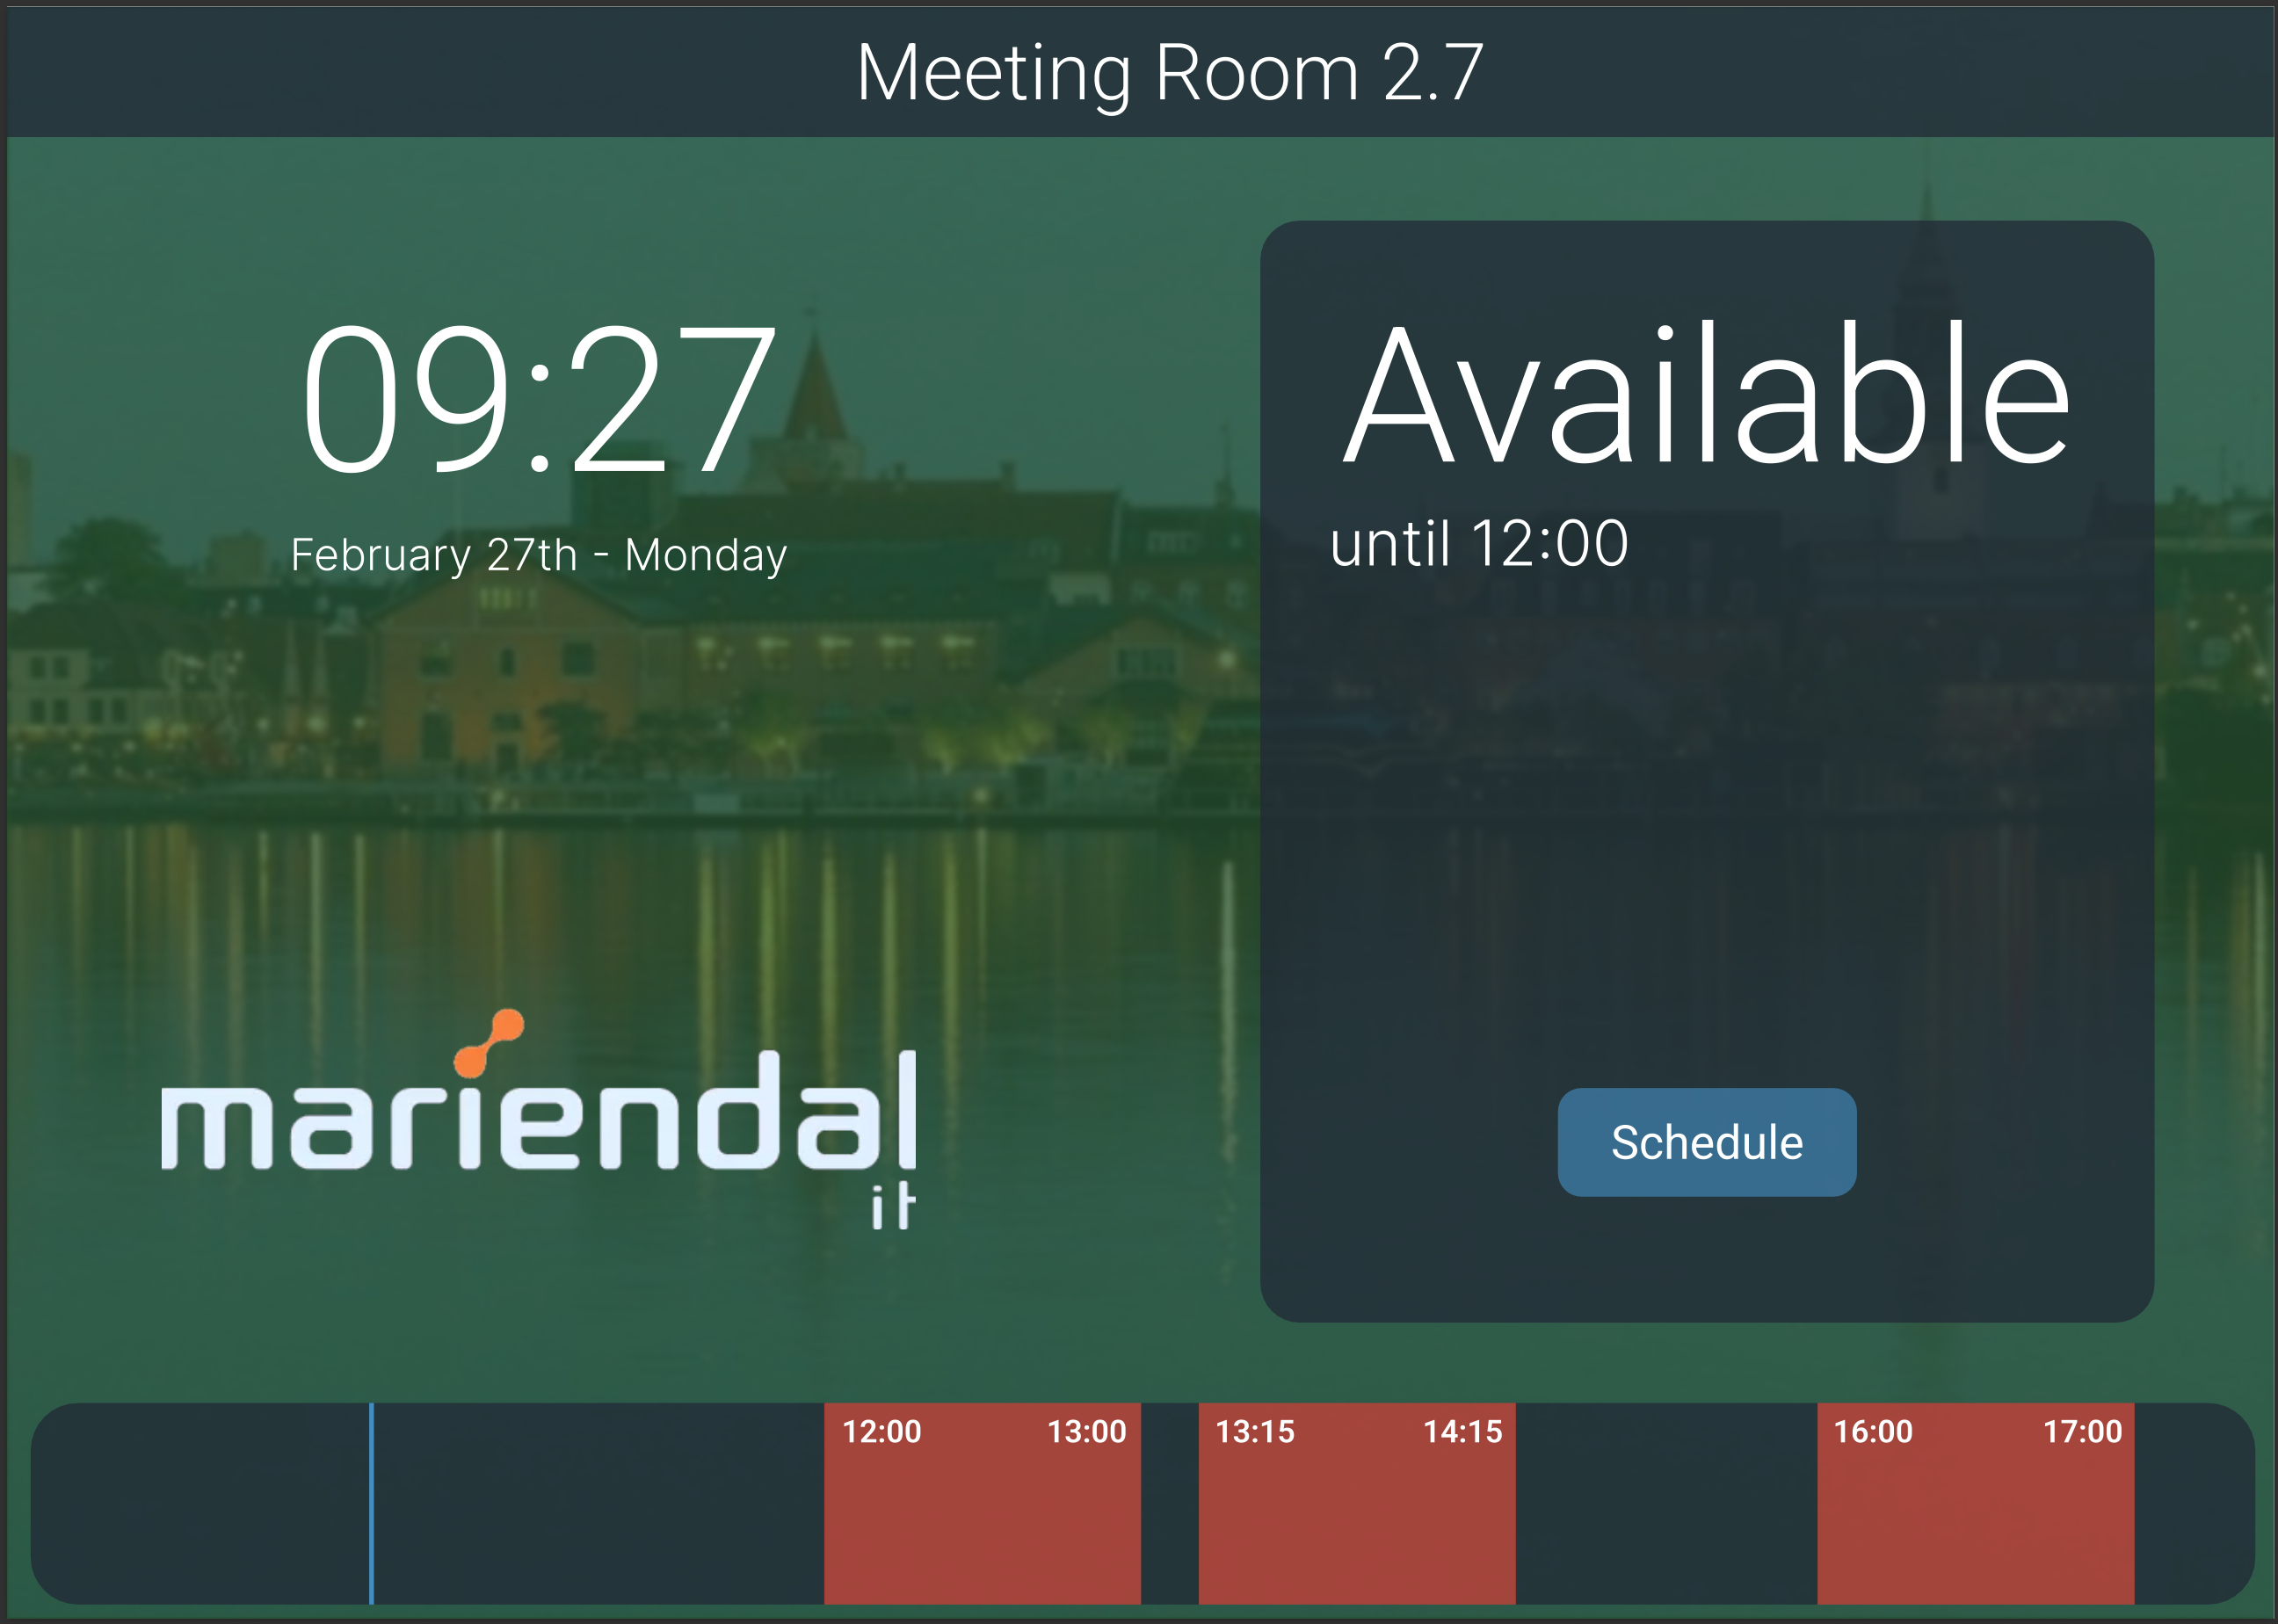
\includegraphics[width=1\textwidth]{images/available_normal.png}
    \caption{The standard view for an available meeting room.}
    \label{fig:available_normal}
  \end{figure}

  \begin{figure}[h!]
    \centering
    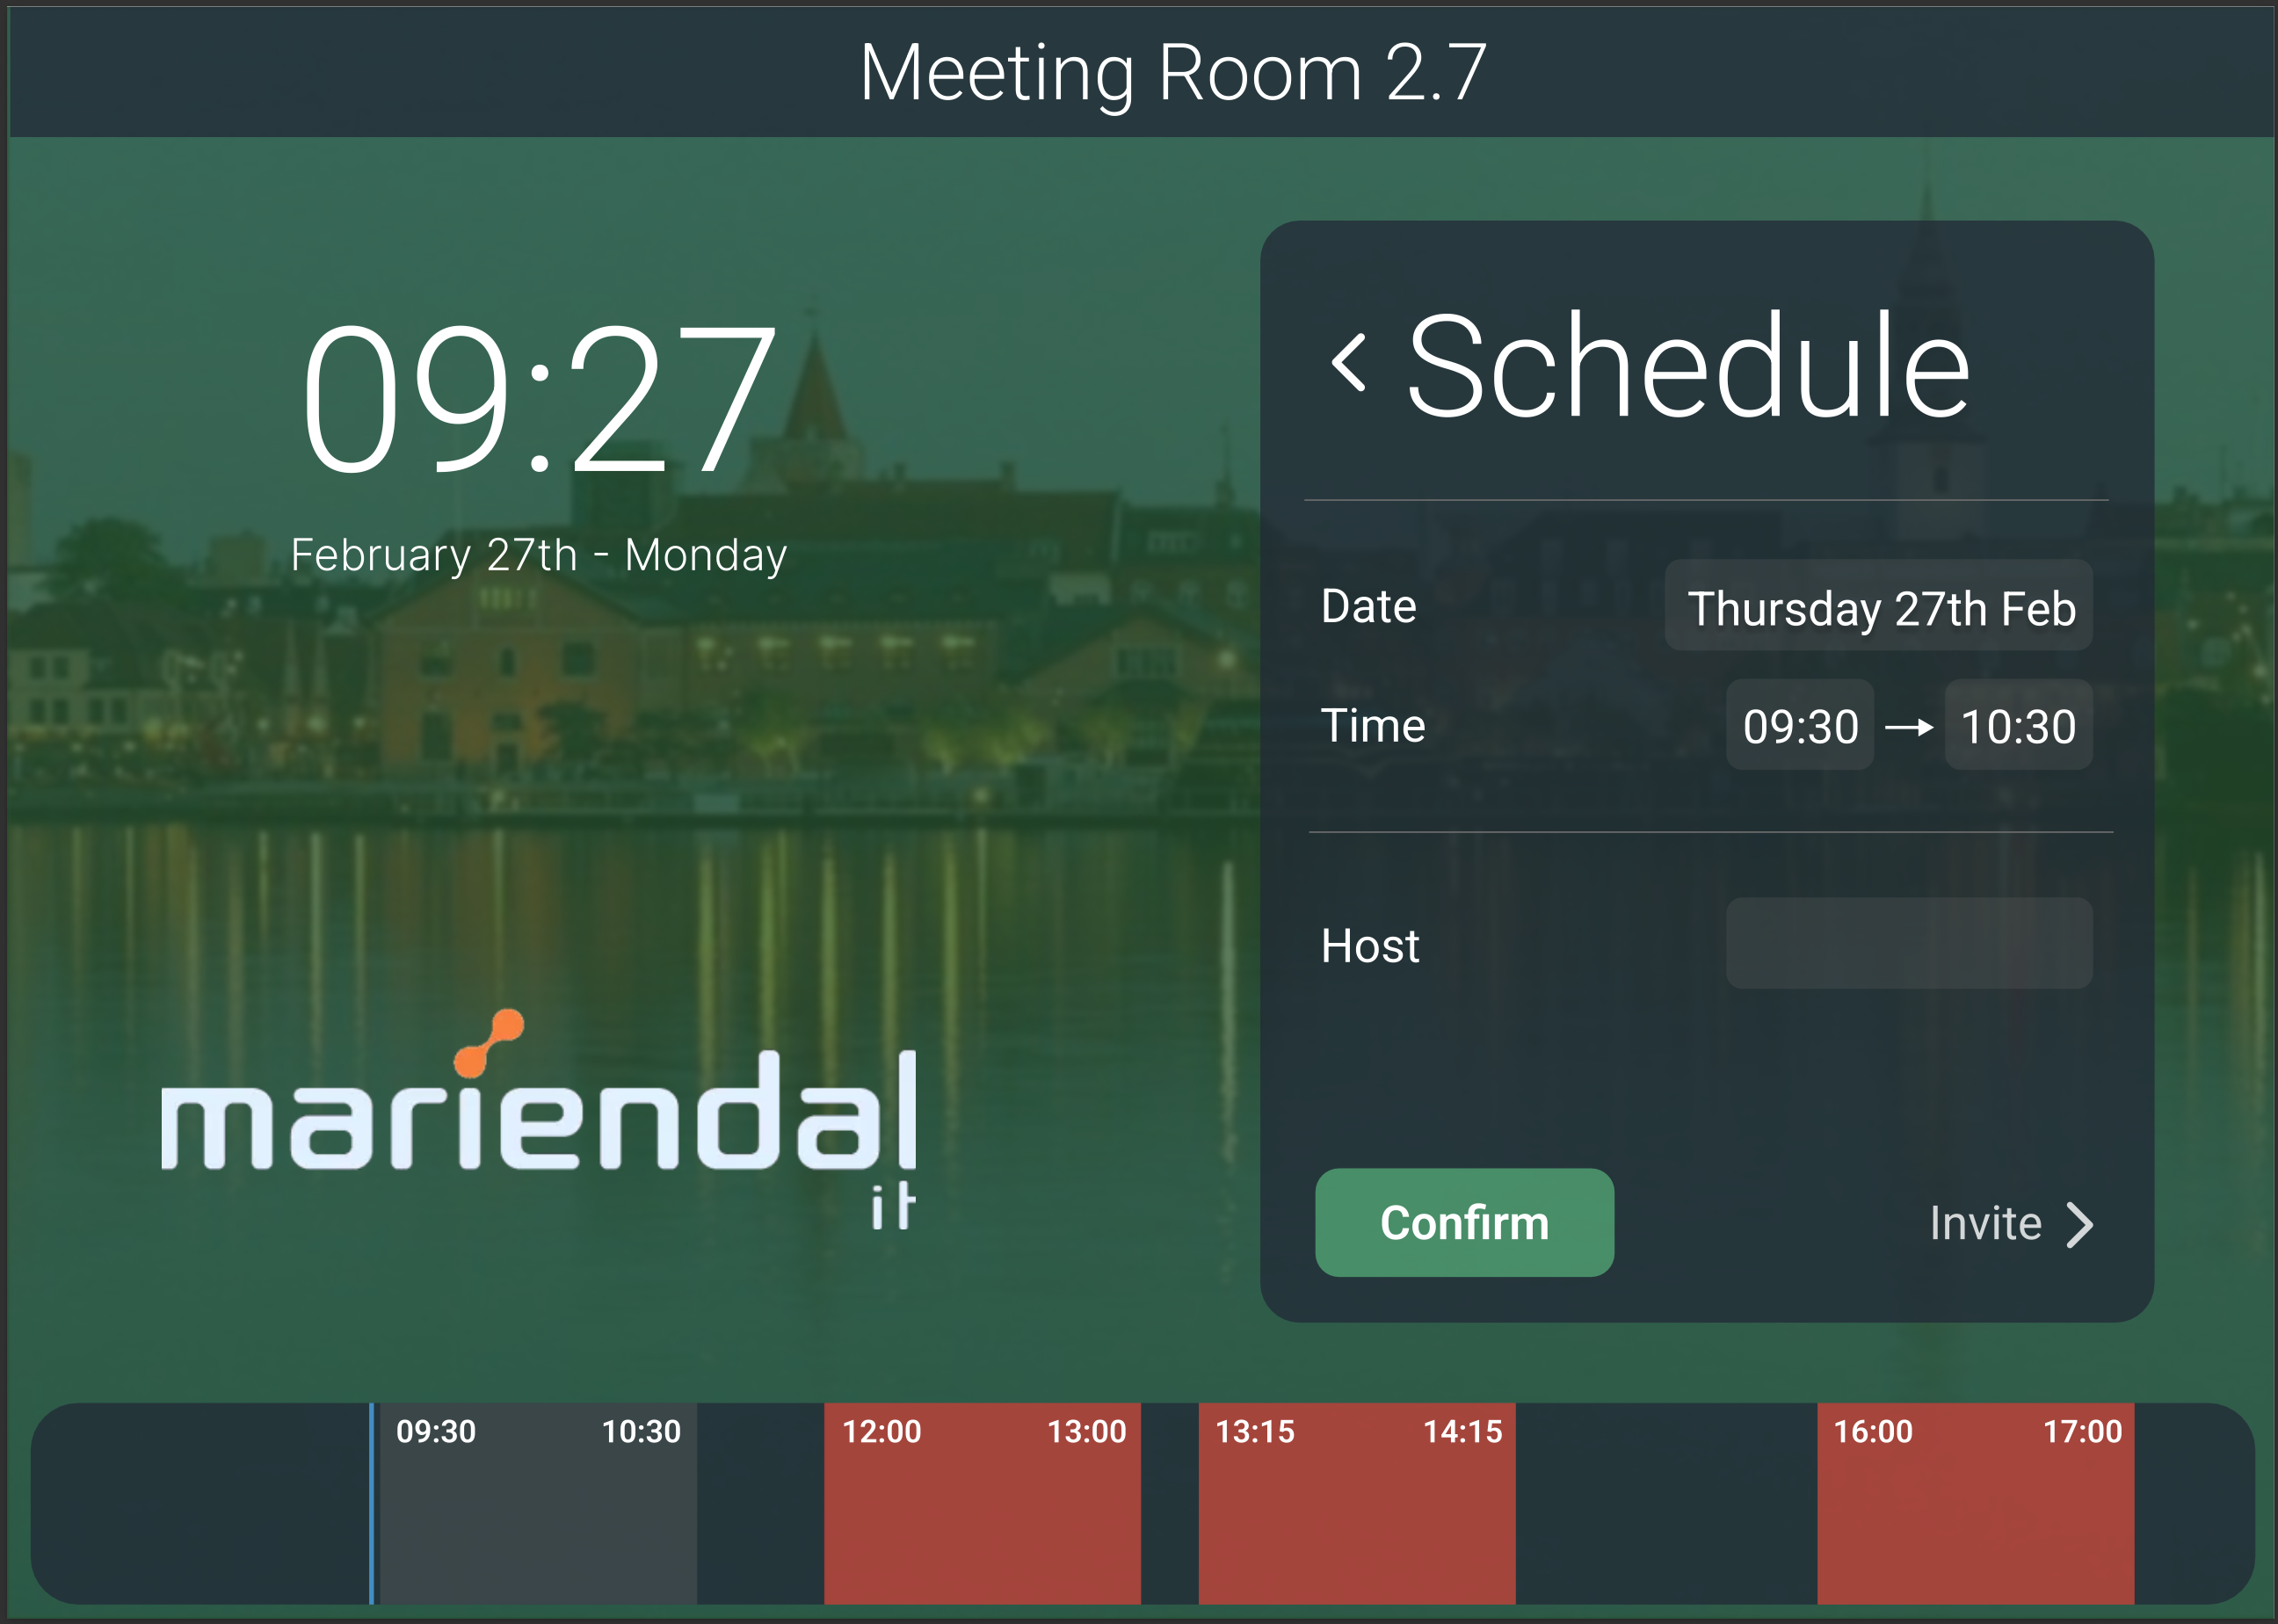
\includegraphics[width=1\textwidth]{images/available_schedule.png}
    \caption{The available view with the schedule meeting action open.}
    \label{fig:available_schedule}
  \end{figure}

  \begin{figure}[h!]
    \centering
    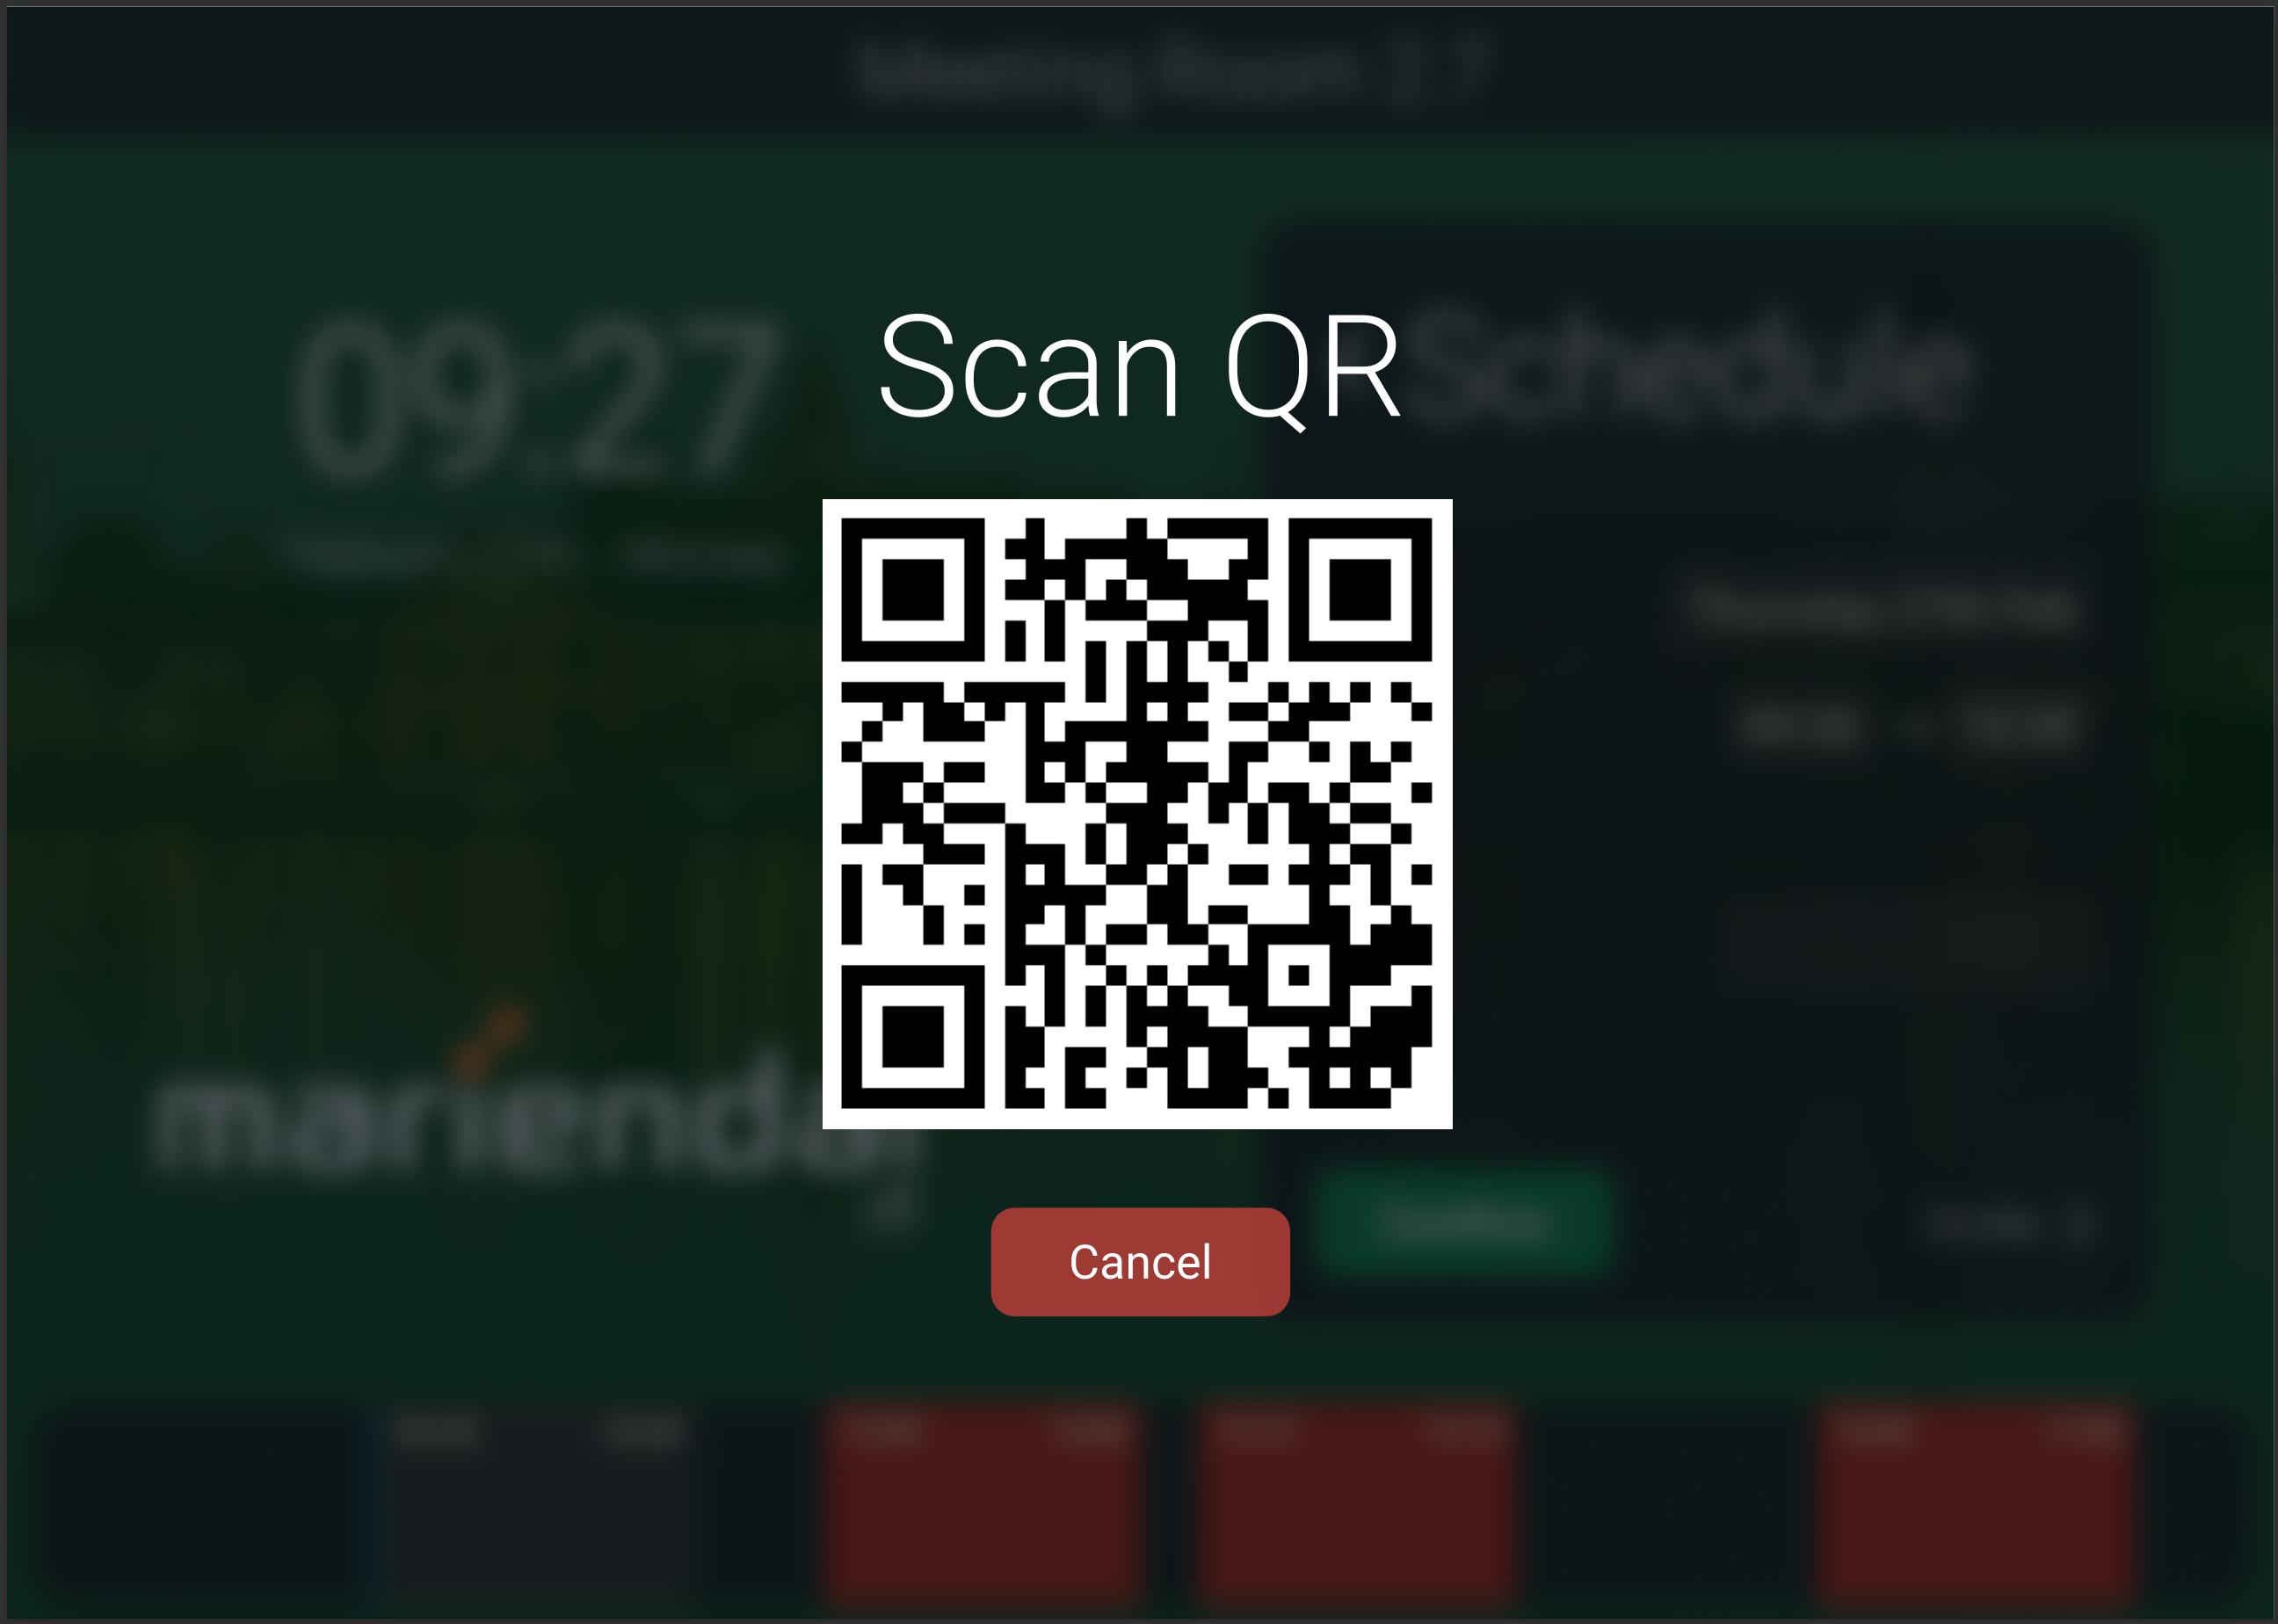
\includegraphics[width=1\textwidth]{images/available_qr.png}
    \caption{The available view with a QR code on top.}
    \label{fig:available_qr}
  \end{figure}

  \begin{figure}[h!]
    \centering
    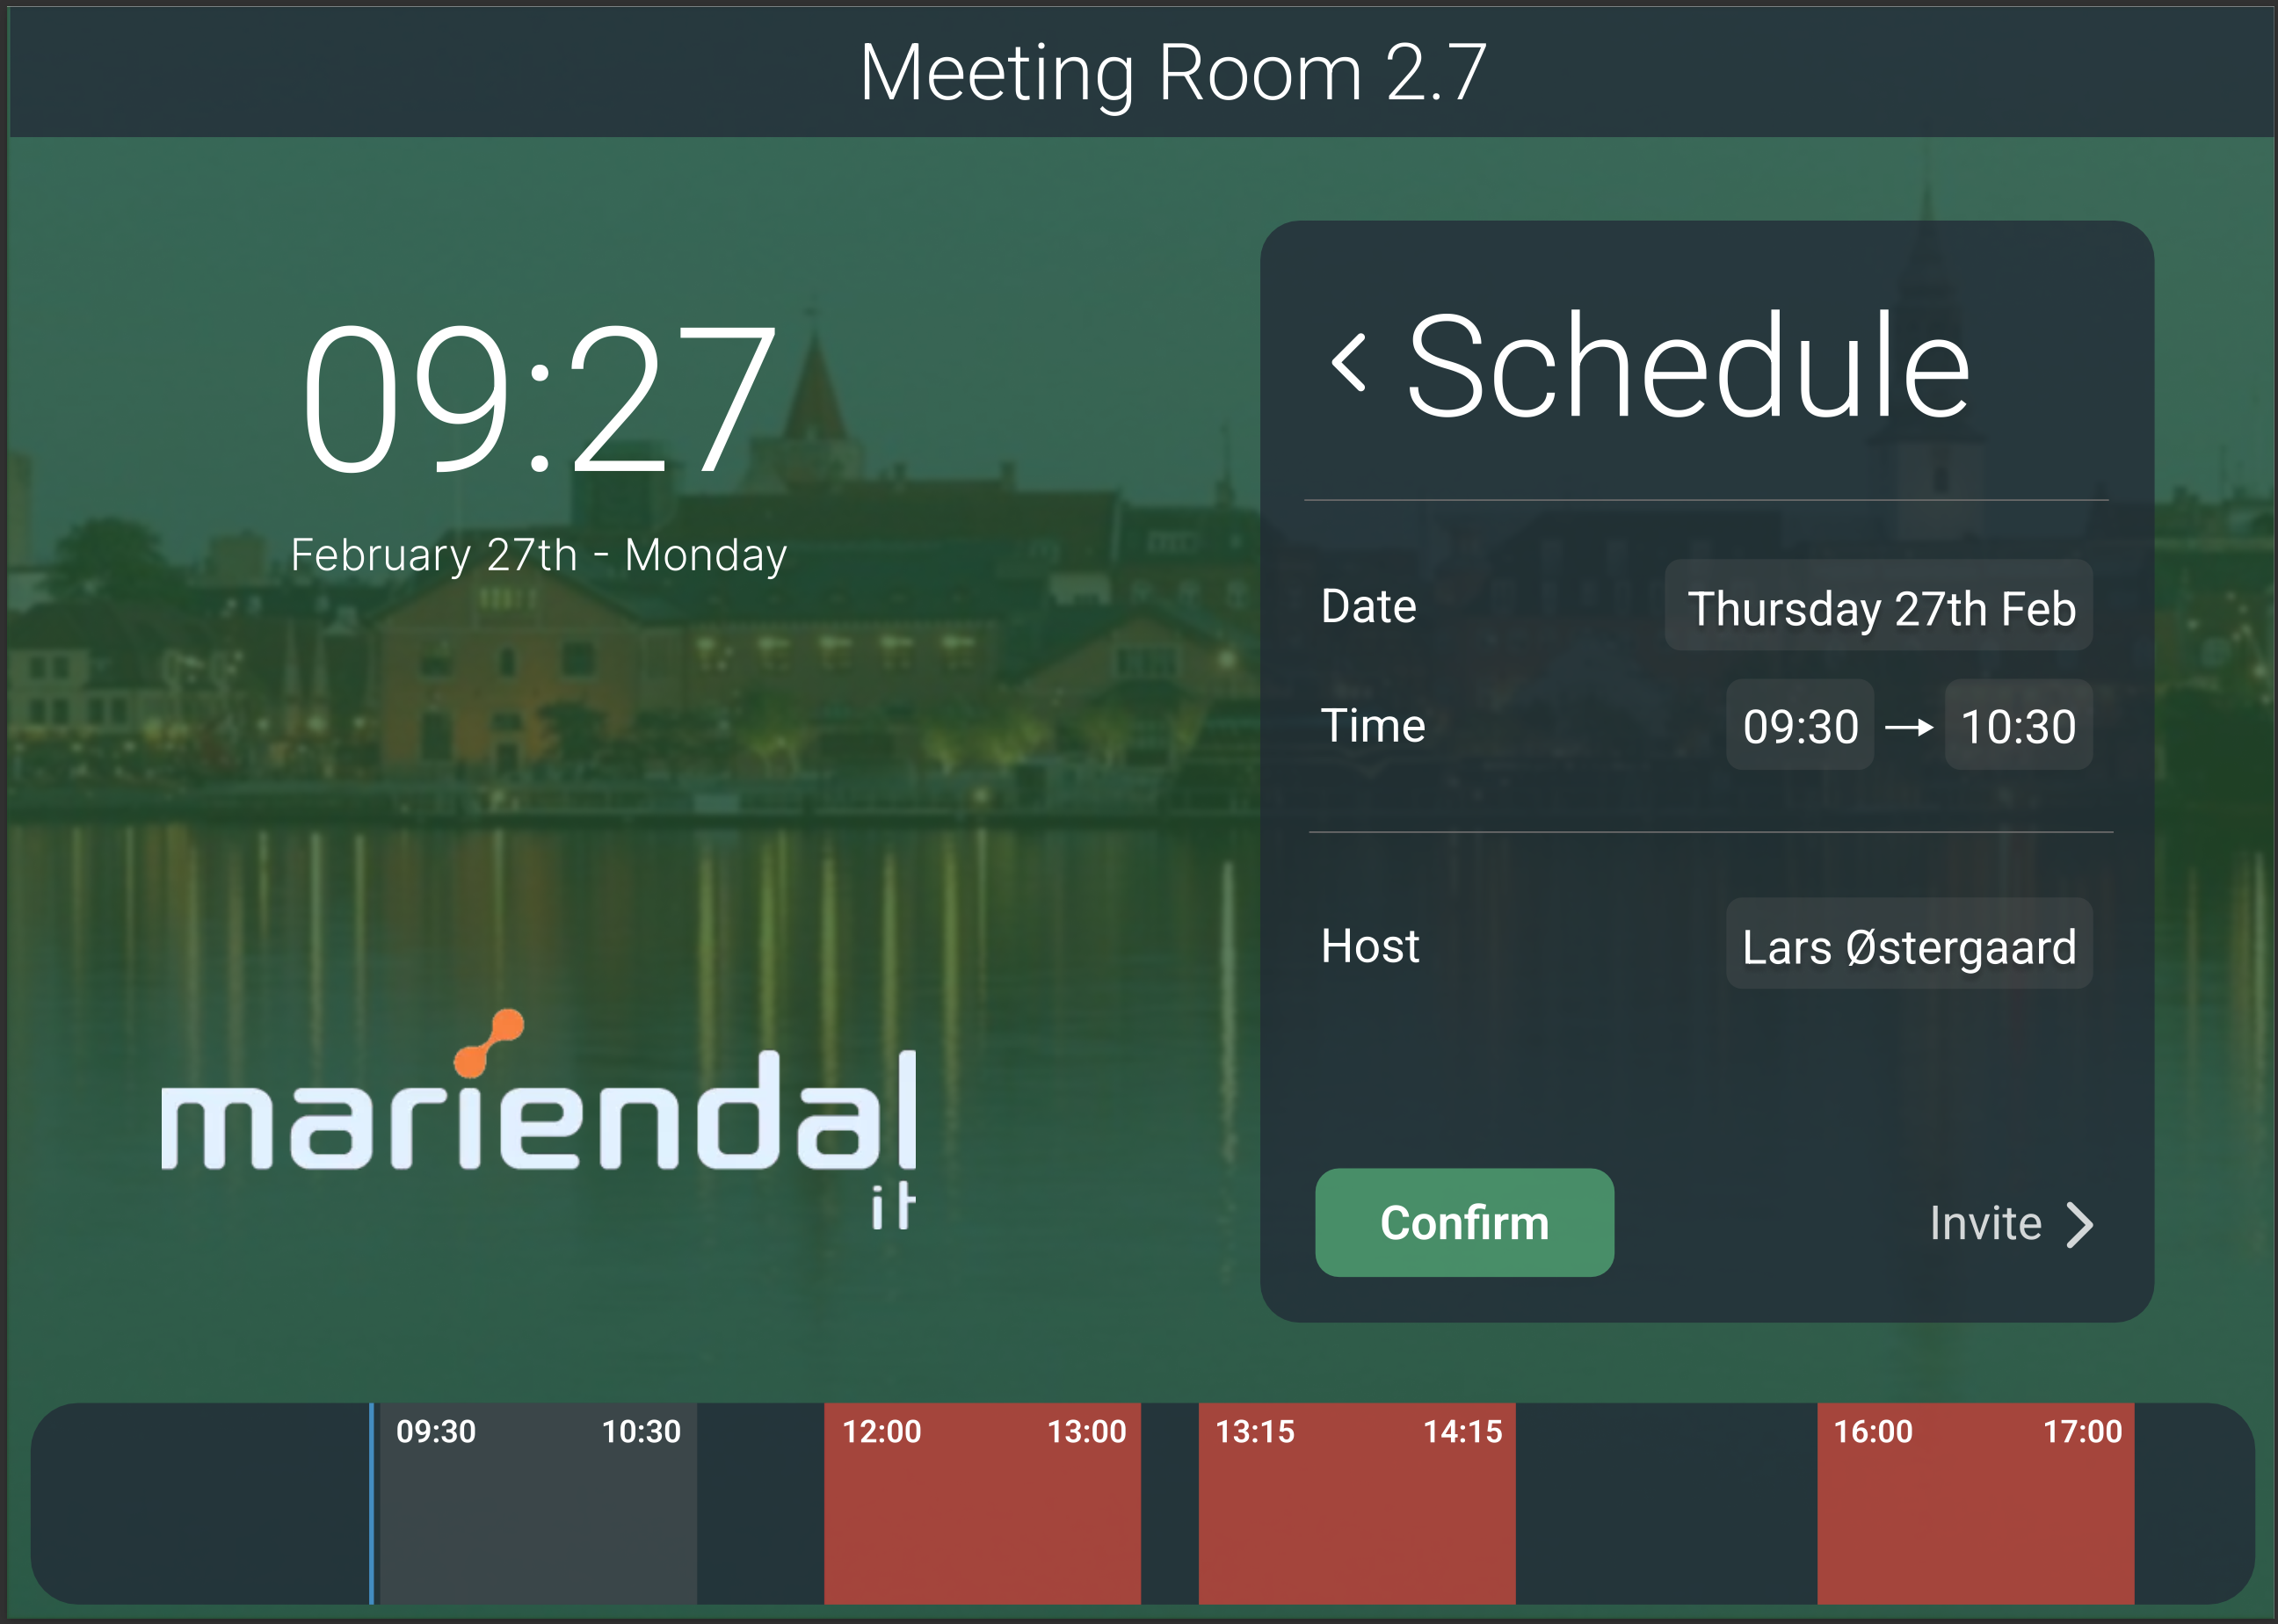
\includegraphics[width=1\textwidth]{images/available_host}
    \caption{The available view with the information required to schedule a new meeting filled in.}
    \label{fig:available_host}
  \end{figure}

  \begin{figure}[h!]
    \centering
    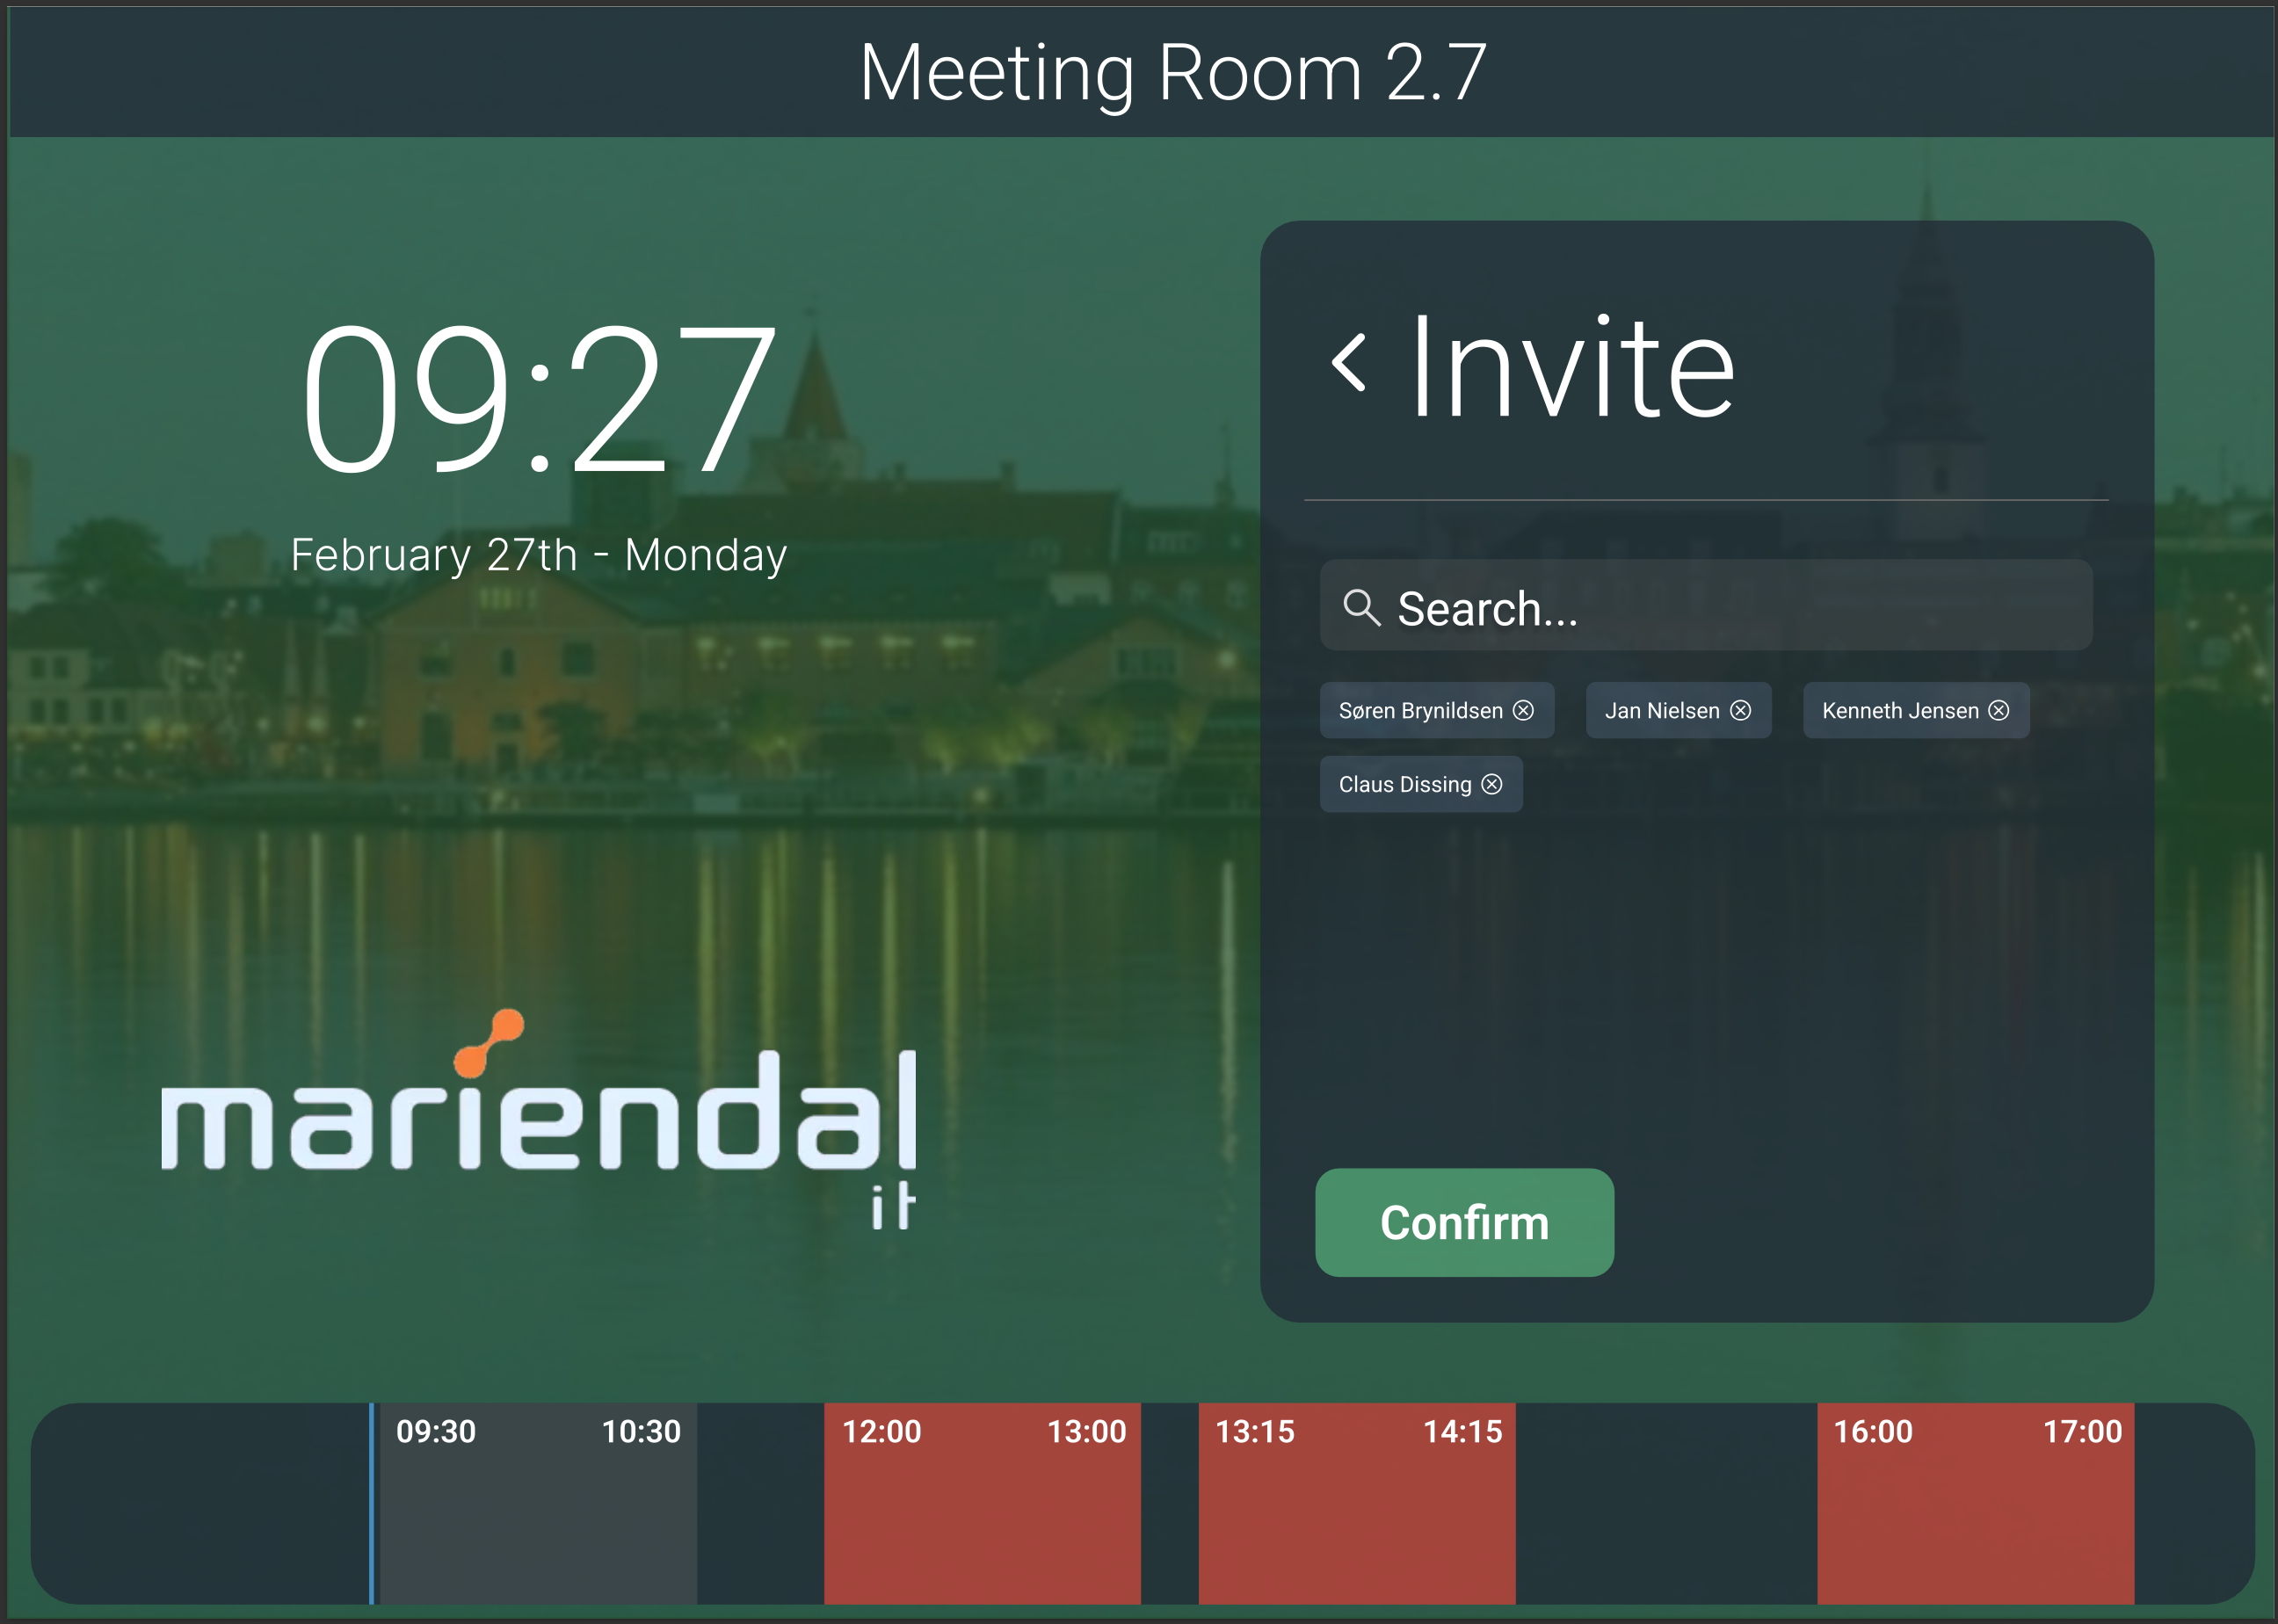
\includegraphics[width=1\textwidth]{images/available_search.png}
    \caption{The available view with the invite to meeting action open on the right.}
    \label{fig:available_search}
  \end{figure}

  \begin{figure}[h!]
    \centering
    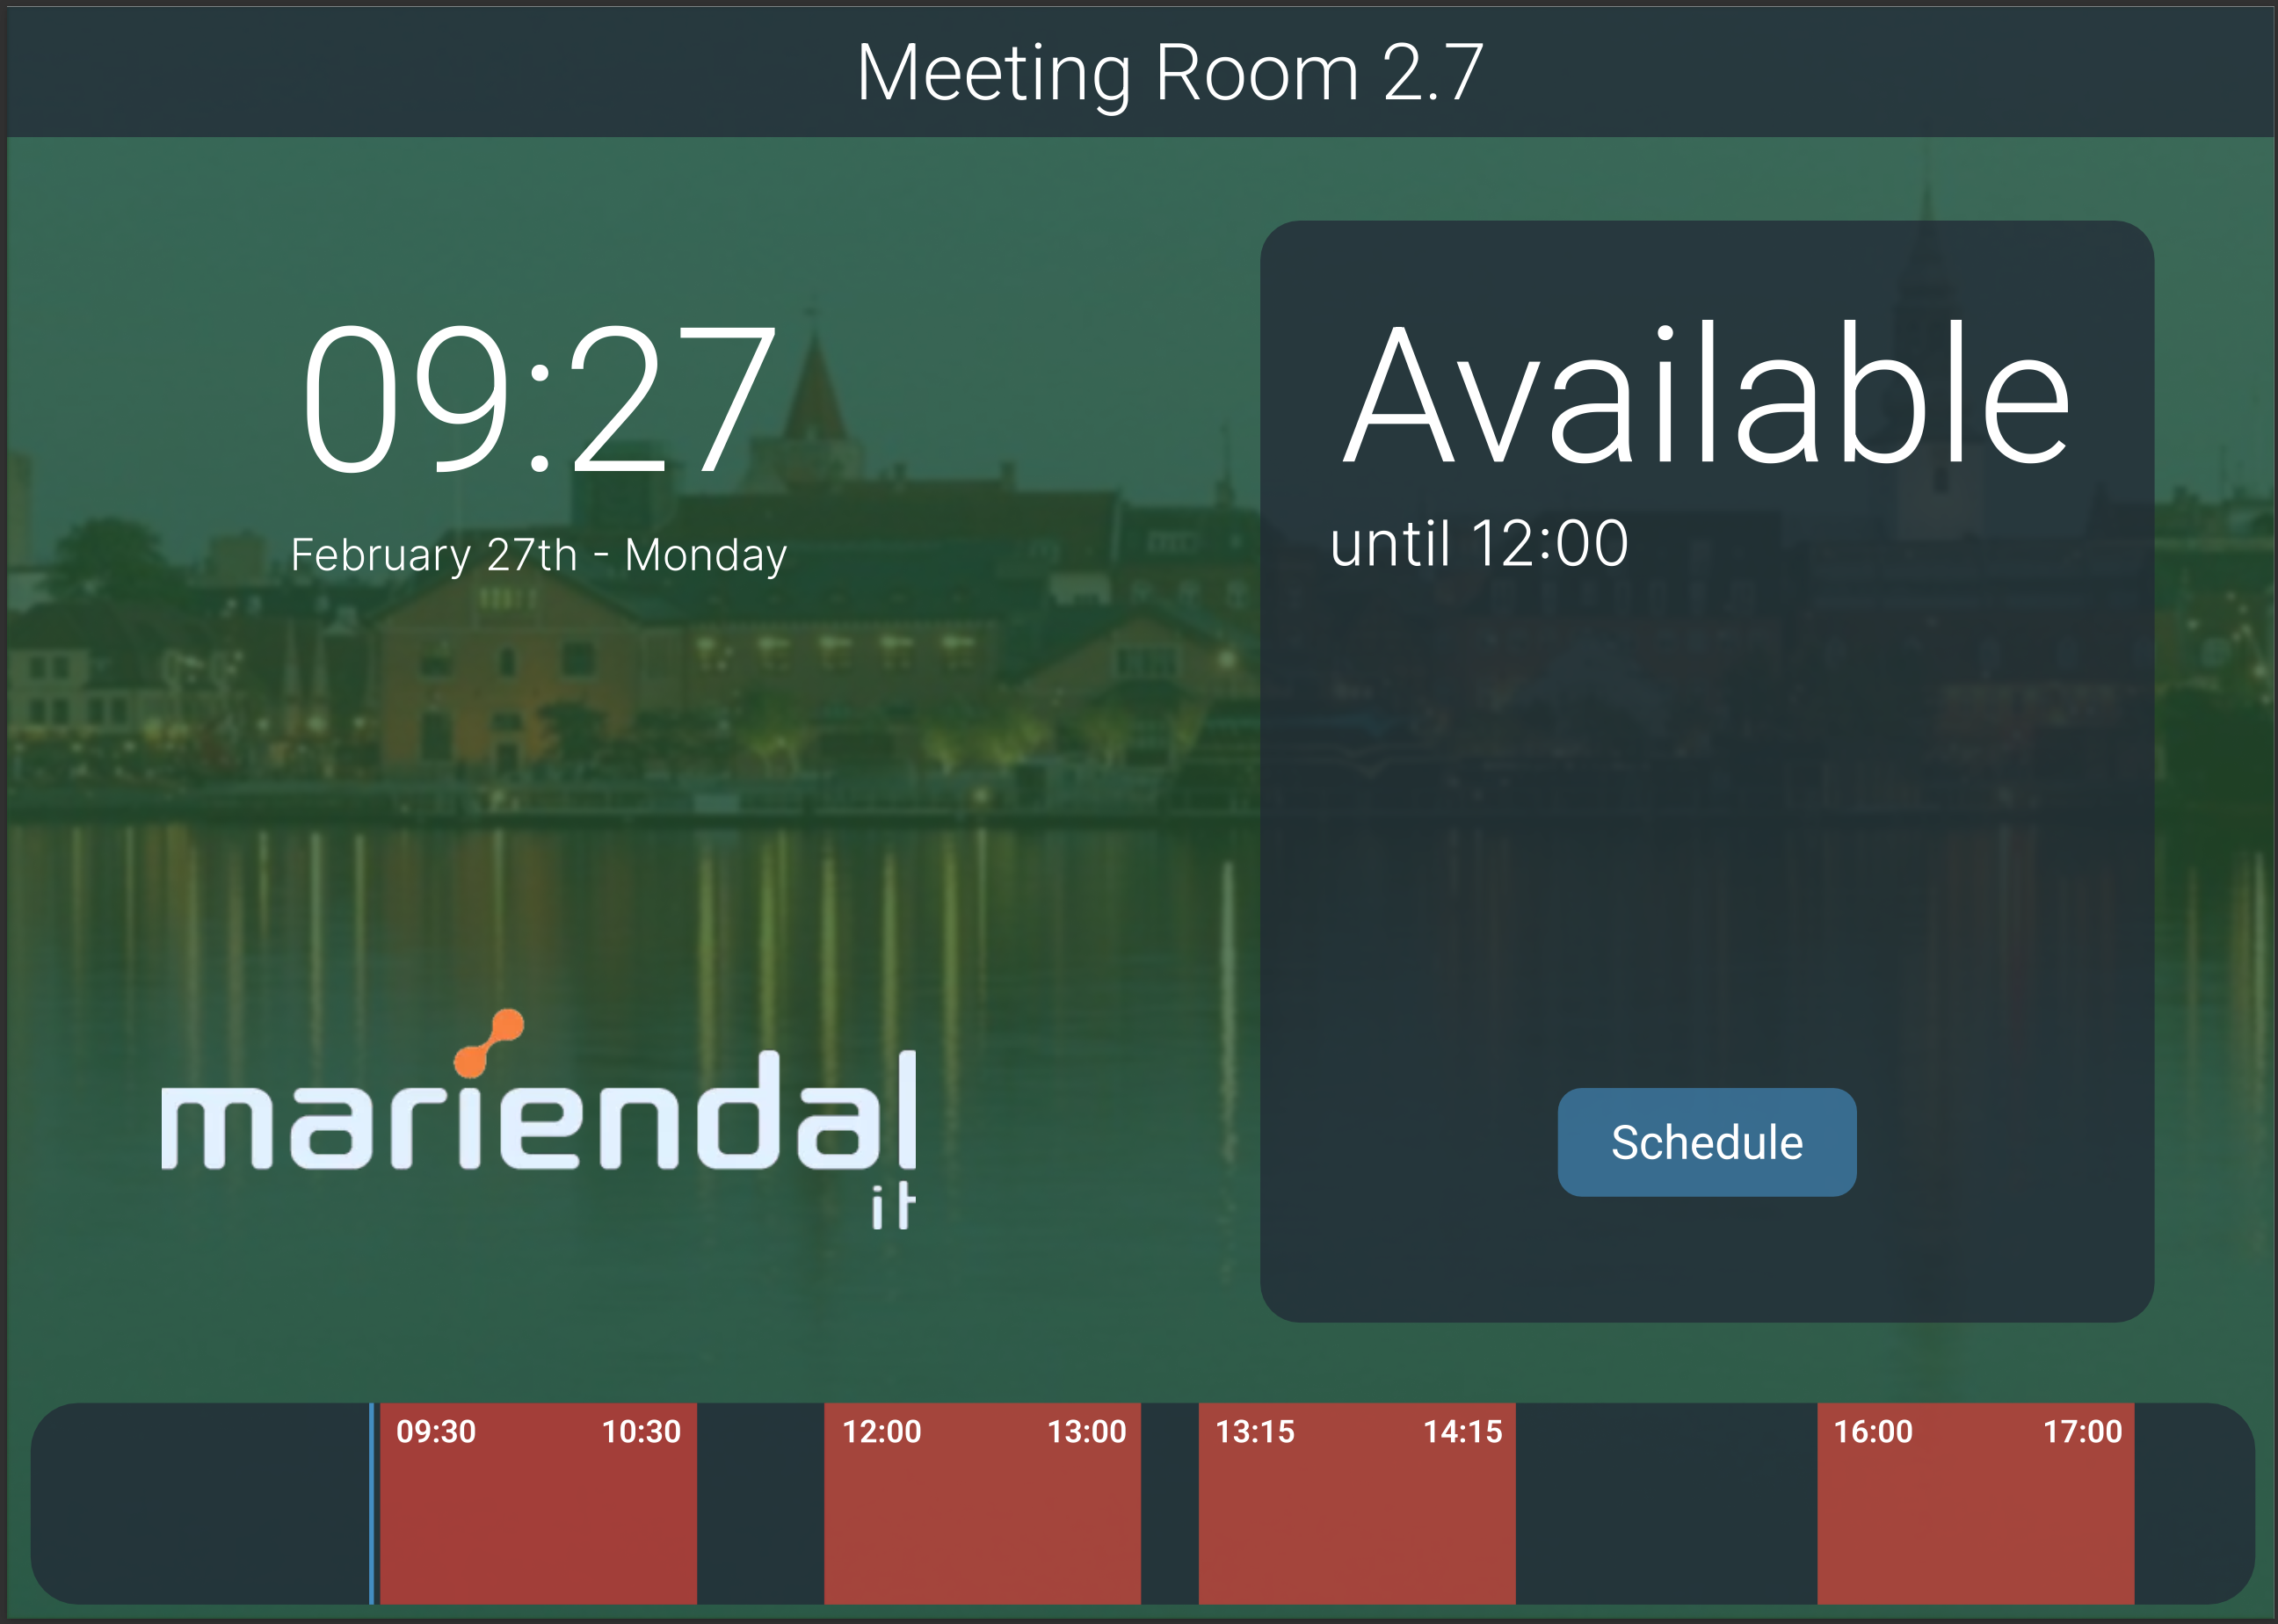
\includegraphics[width=1\textwidth]{images/available_added.png}
    \caption{The available view with the newly added meeting at the bottom.}
    \label{fig:available_added}
  \end{figure}

  \begin{figure}[h!]
    \centering
    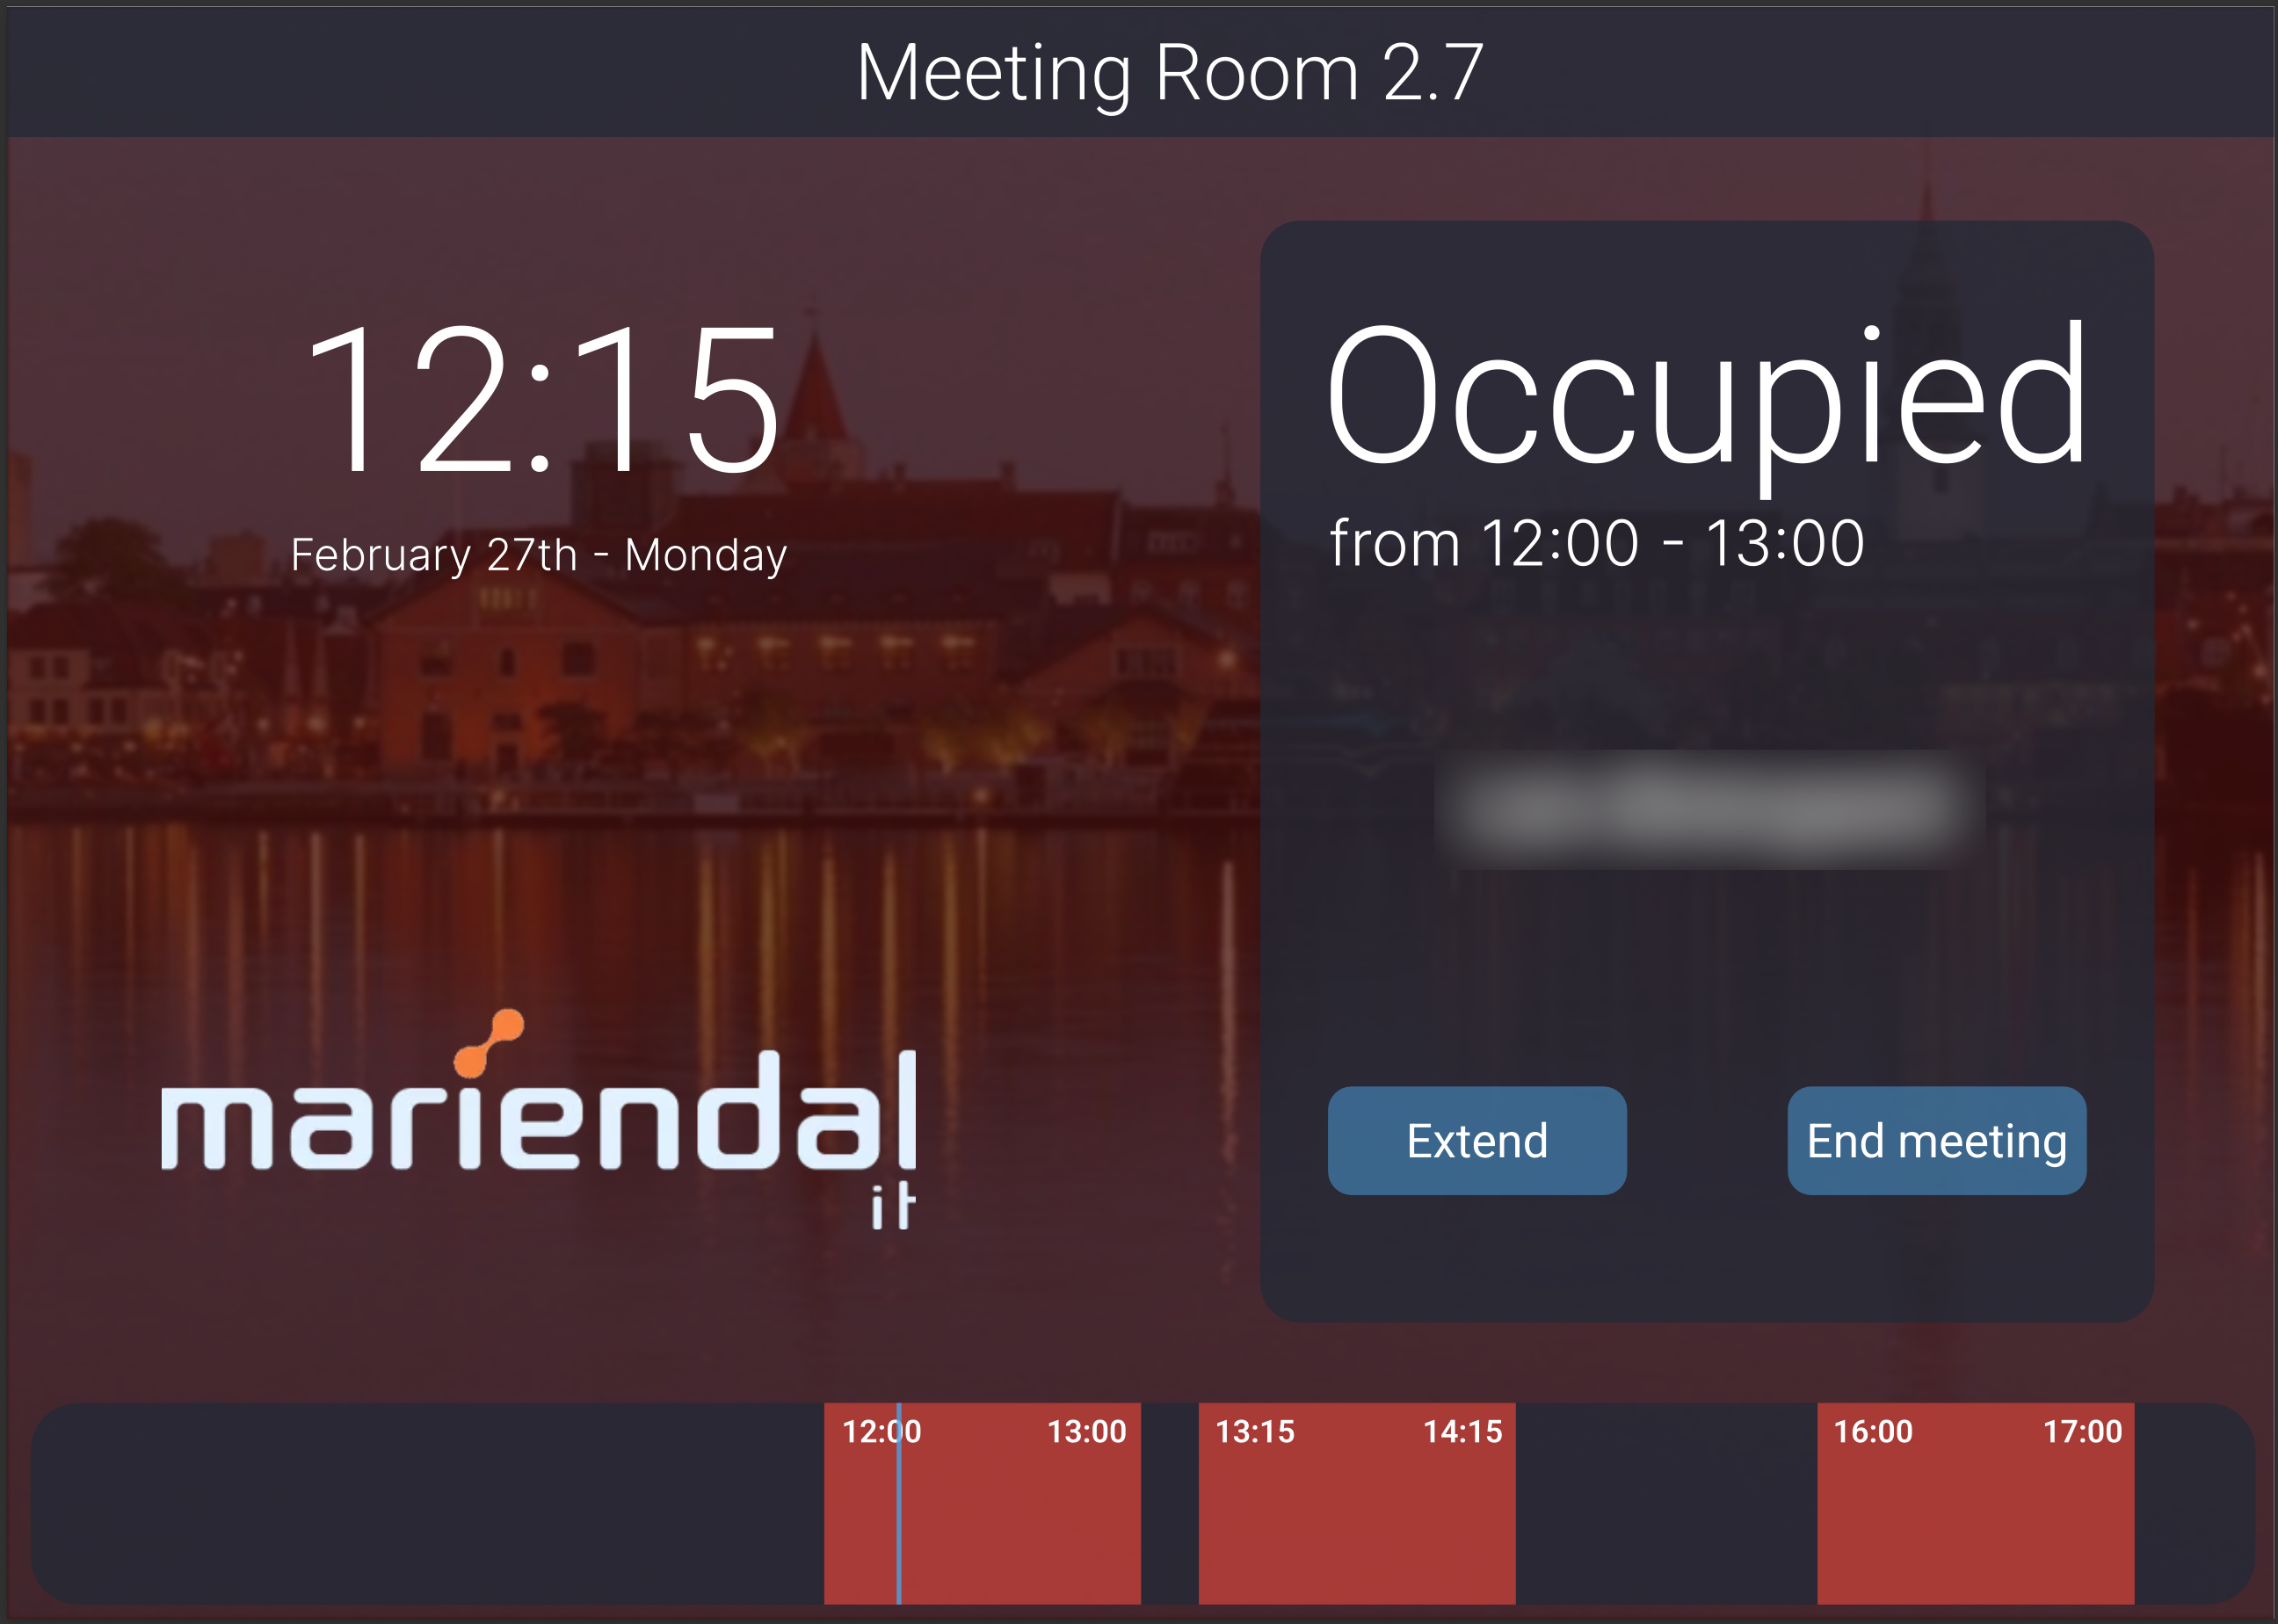
\includegraphics[width=1\textwidth]{images/occupied_normal.png}
    \caption{The standard view for an occupied meeting room.}
    \label{fig:occupied_normal}
  \end{figure}

  \begin{figure}[h!]
    \centering
    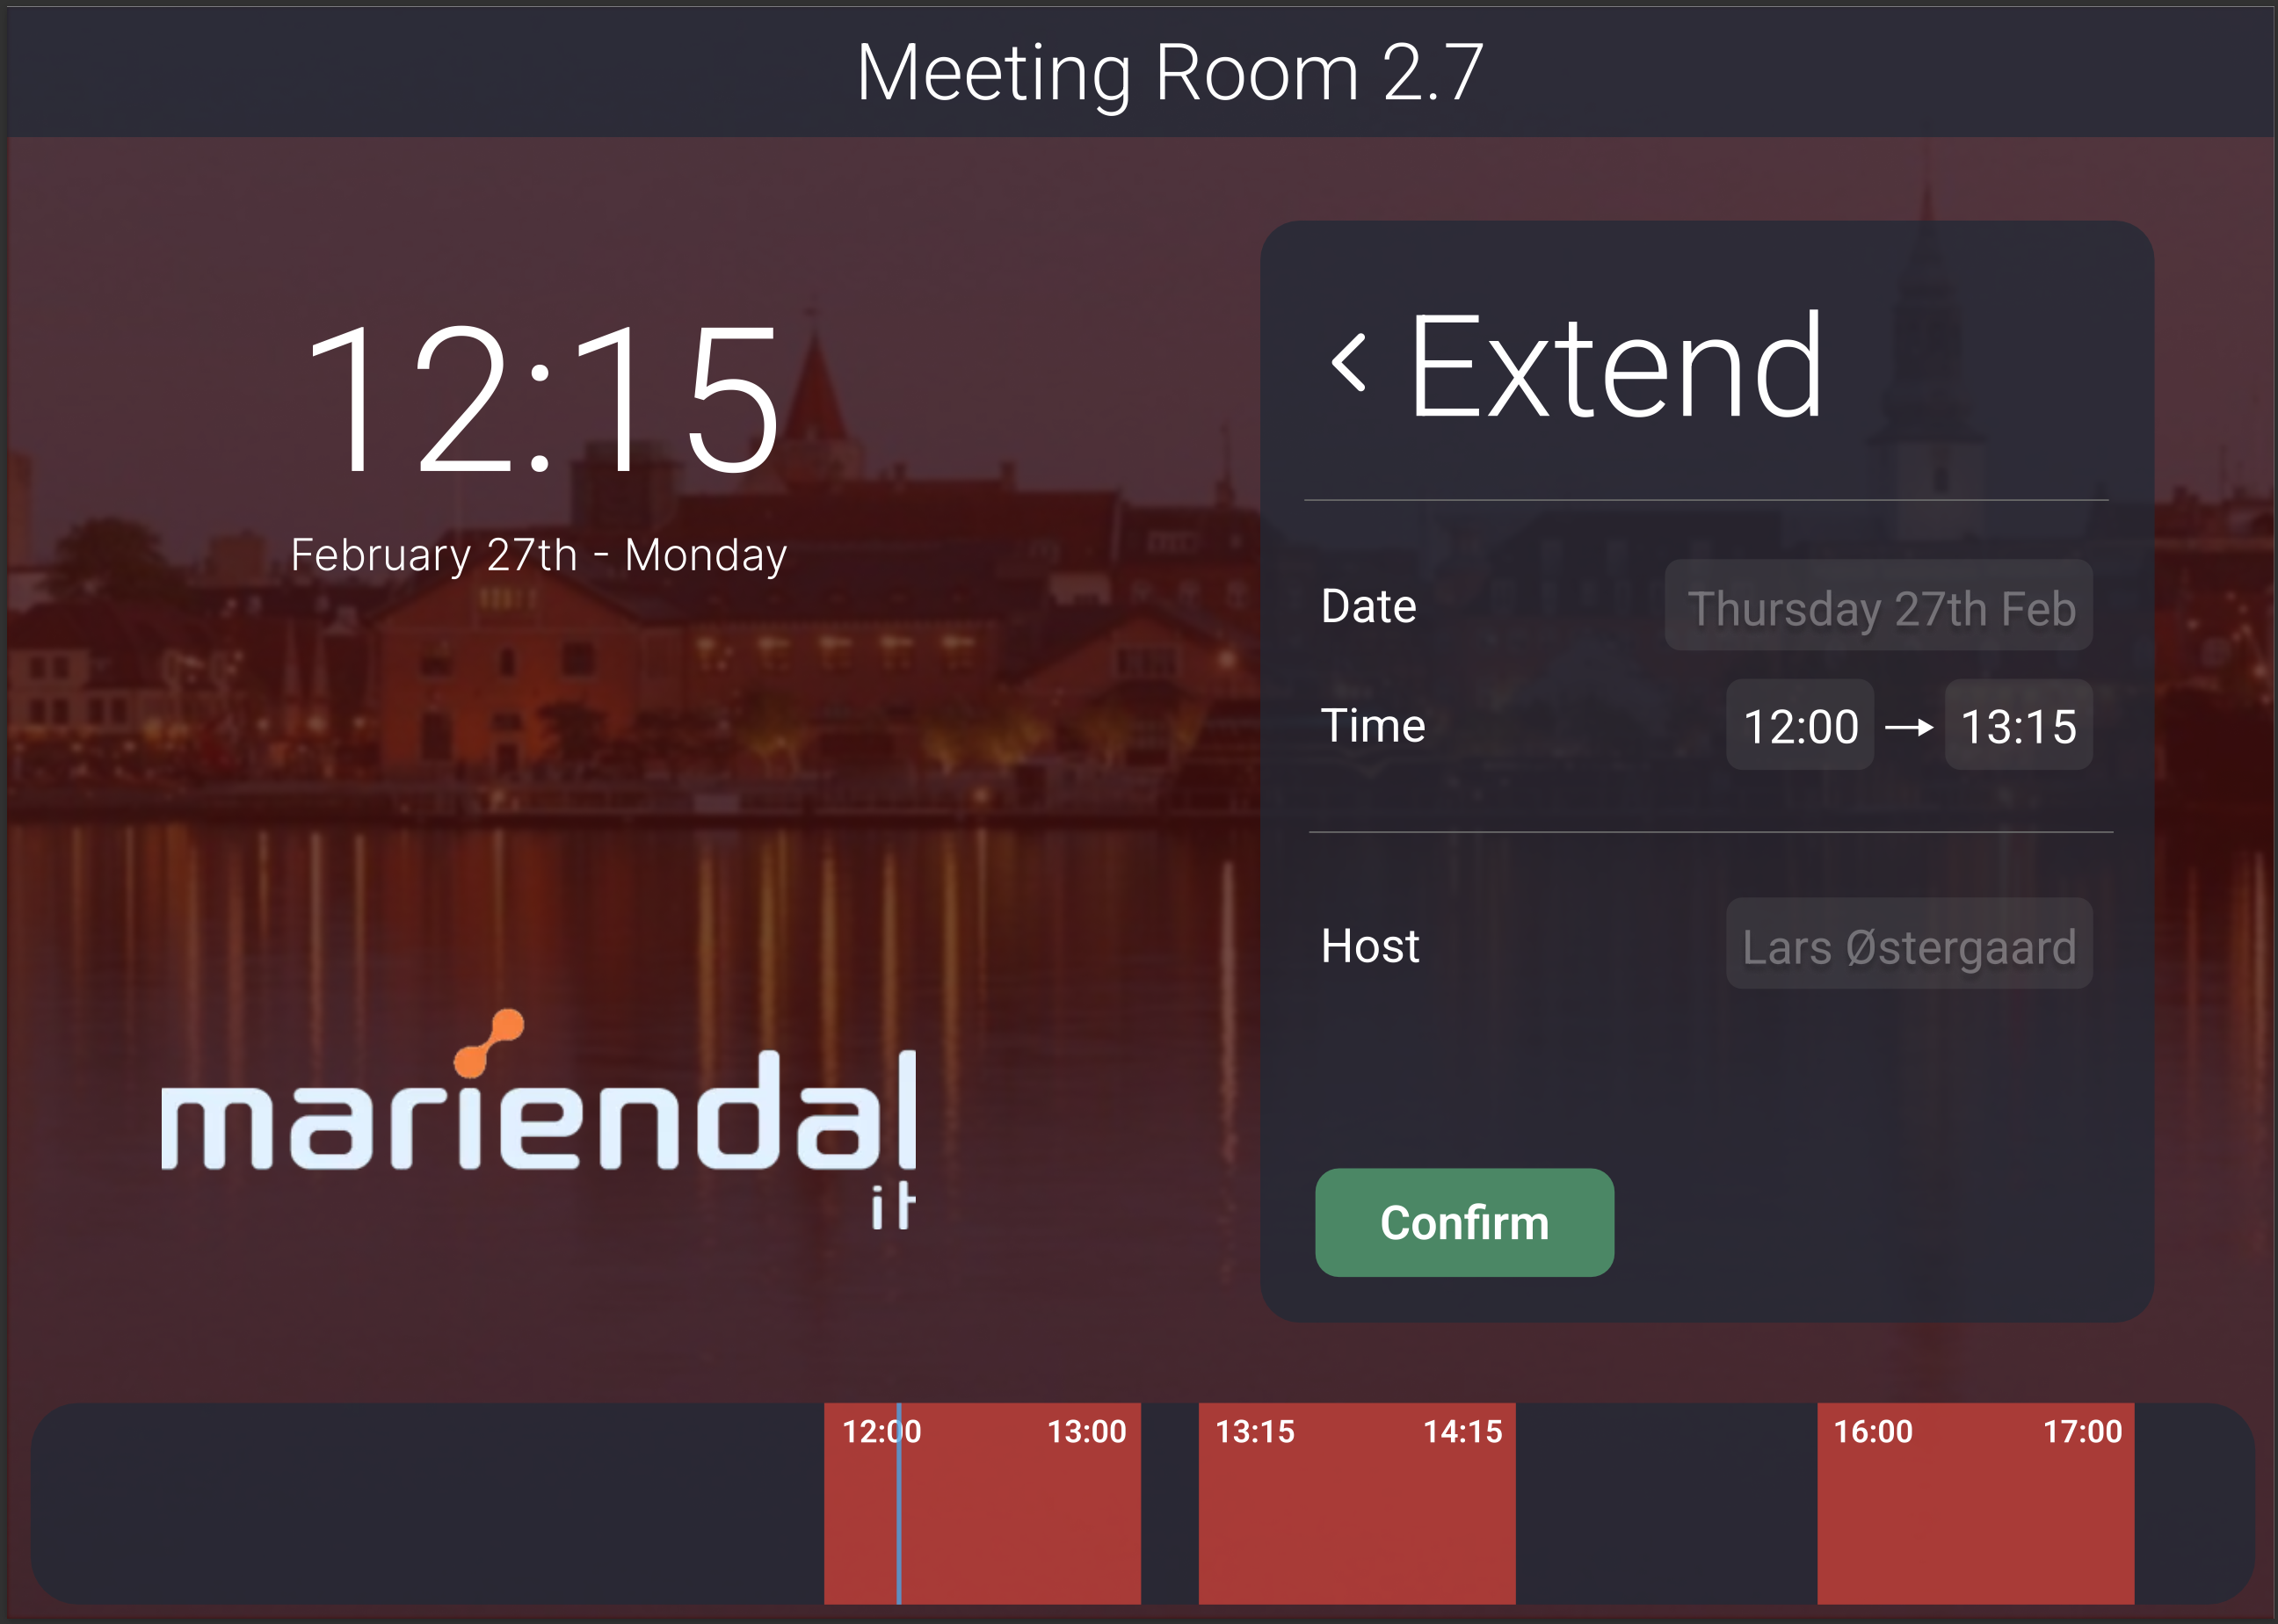
\includegraphics[width=1\textwidth]{images/occupied_extend.png}
    \caption{The occupied view with the extend action open on the right side.}
    \label{fig:occupied_extend}
  \end{figure}

  \begin{figure}[h!]
    \centering
    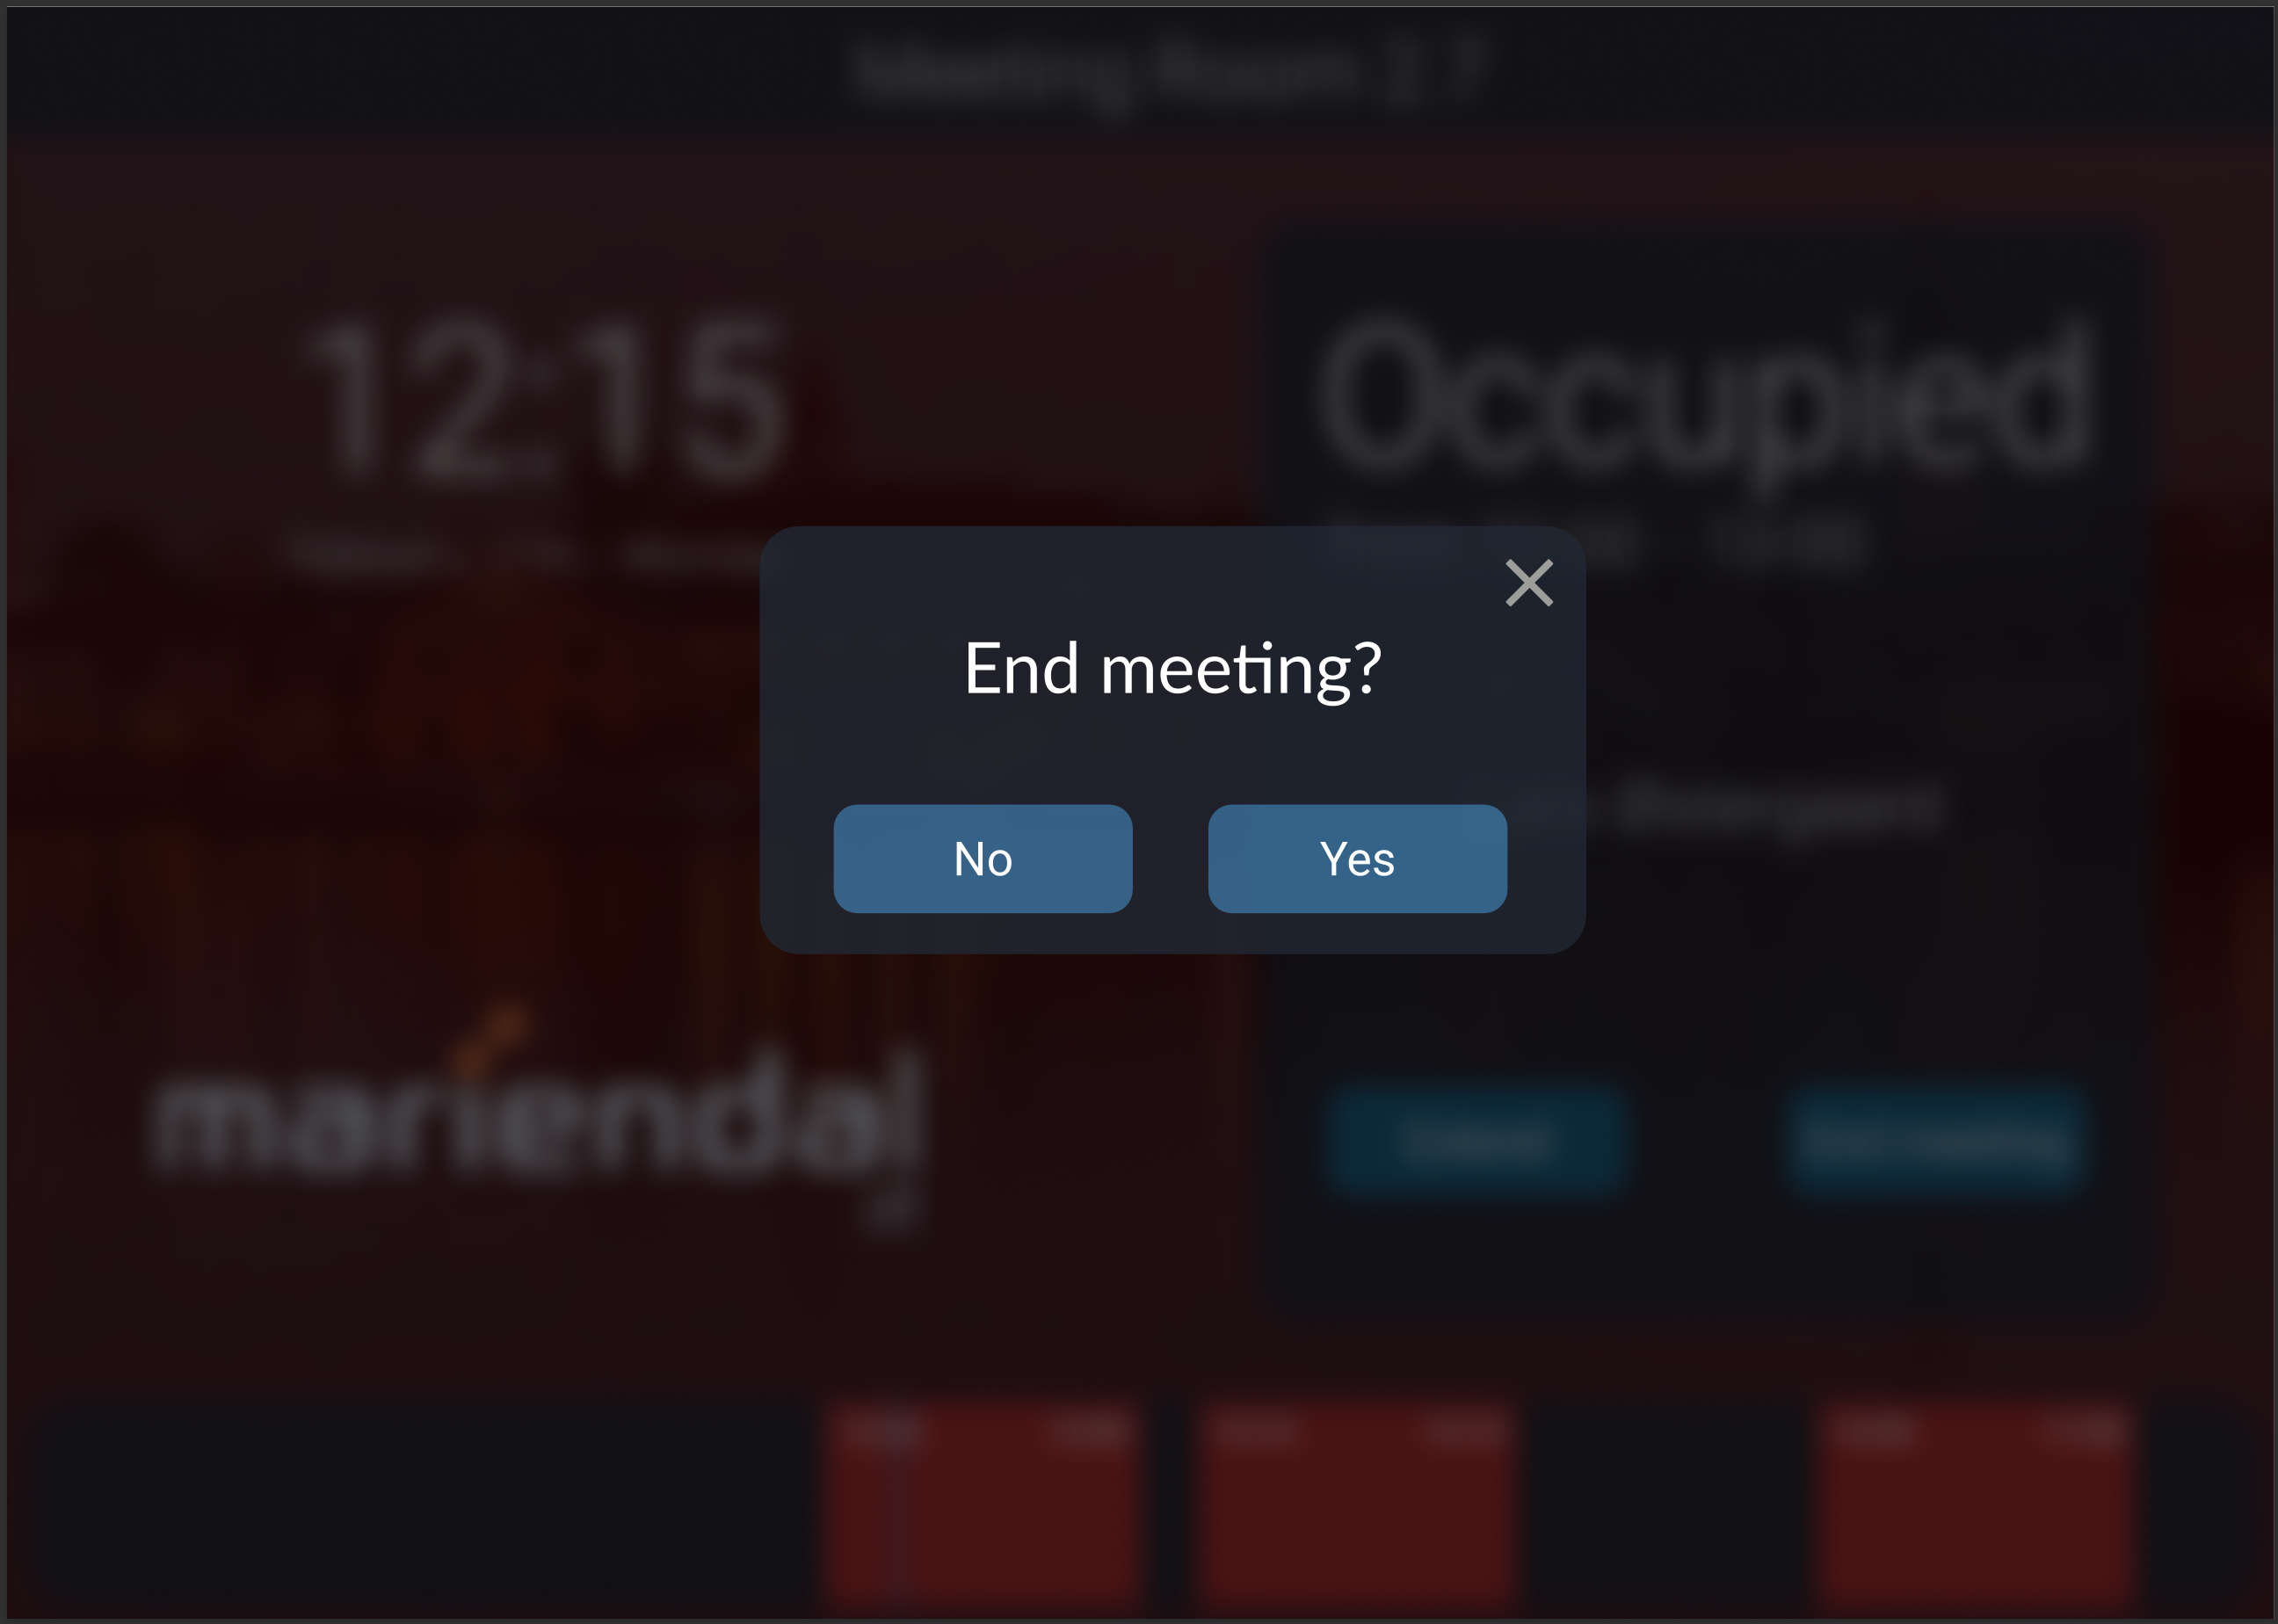
\includegraphics[width=1\textwidth]{images/occupied_end_confirm.png}
    \caption{The occupied view with a confirmation for ending the meeting early on top.}
    \label{fig:occupied_end}
  \end{figure}

  \begin{figure}[h!]
    \centering
    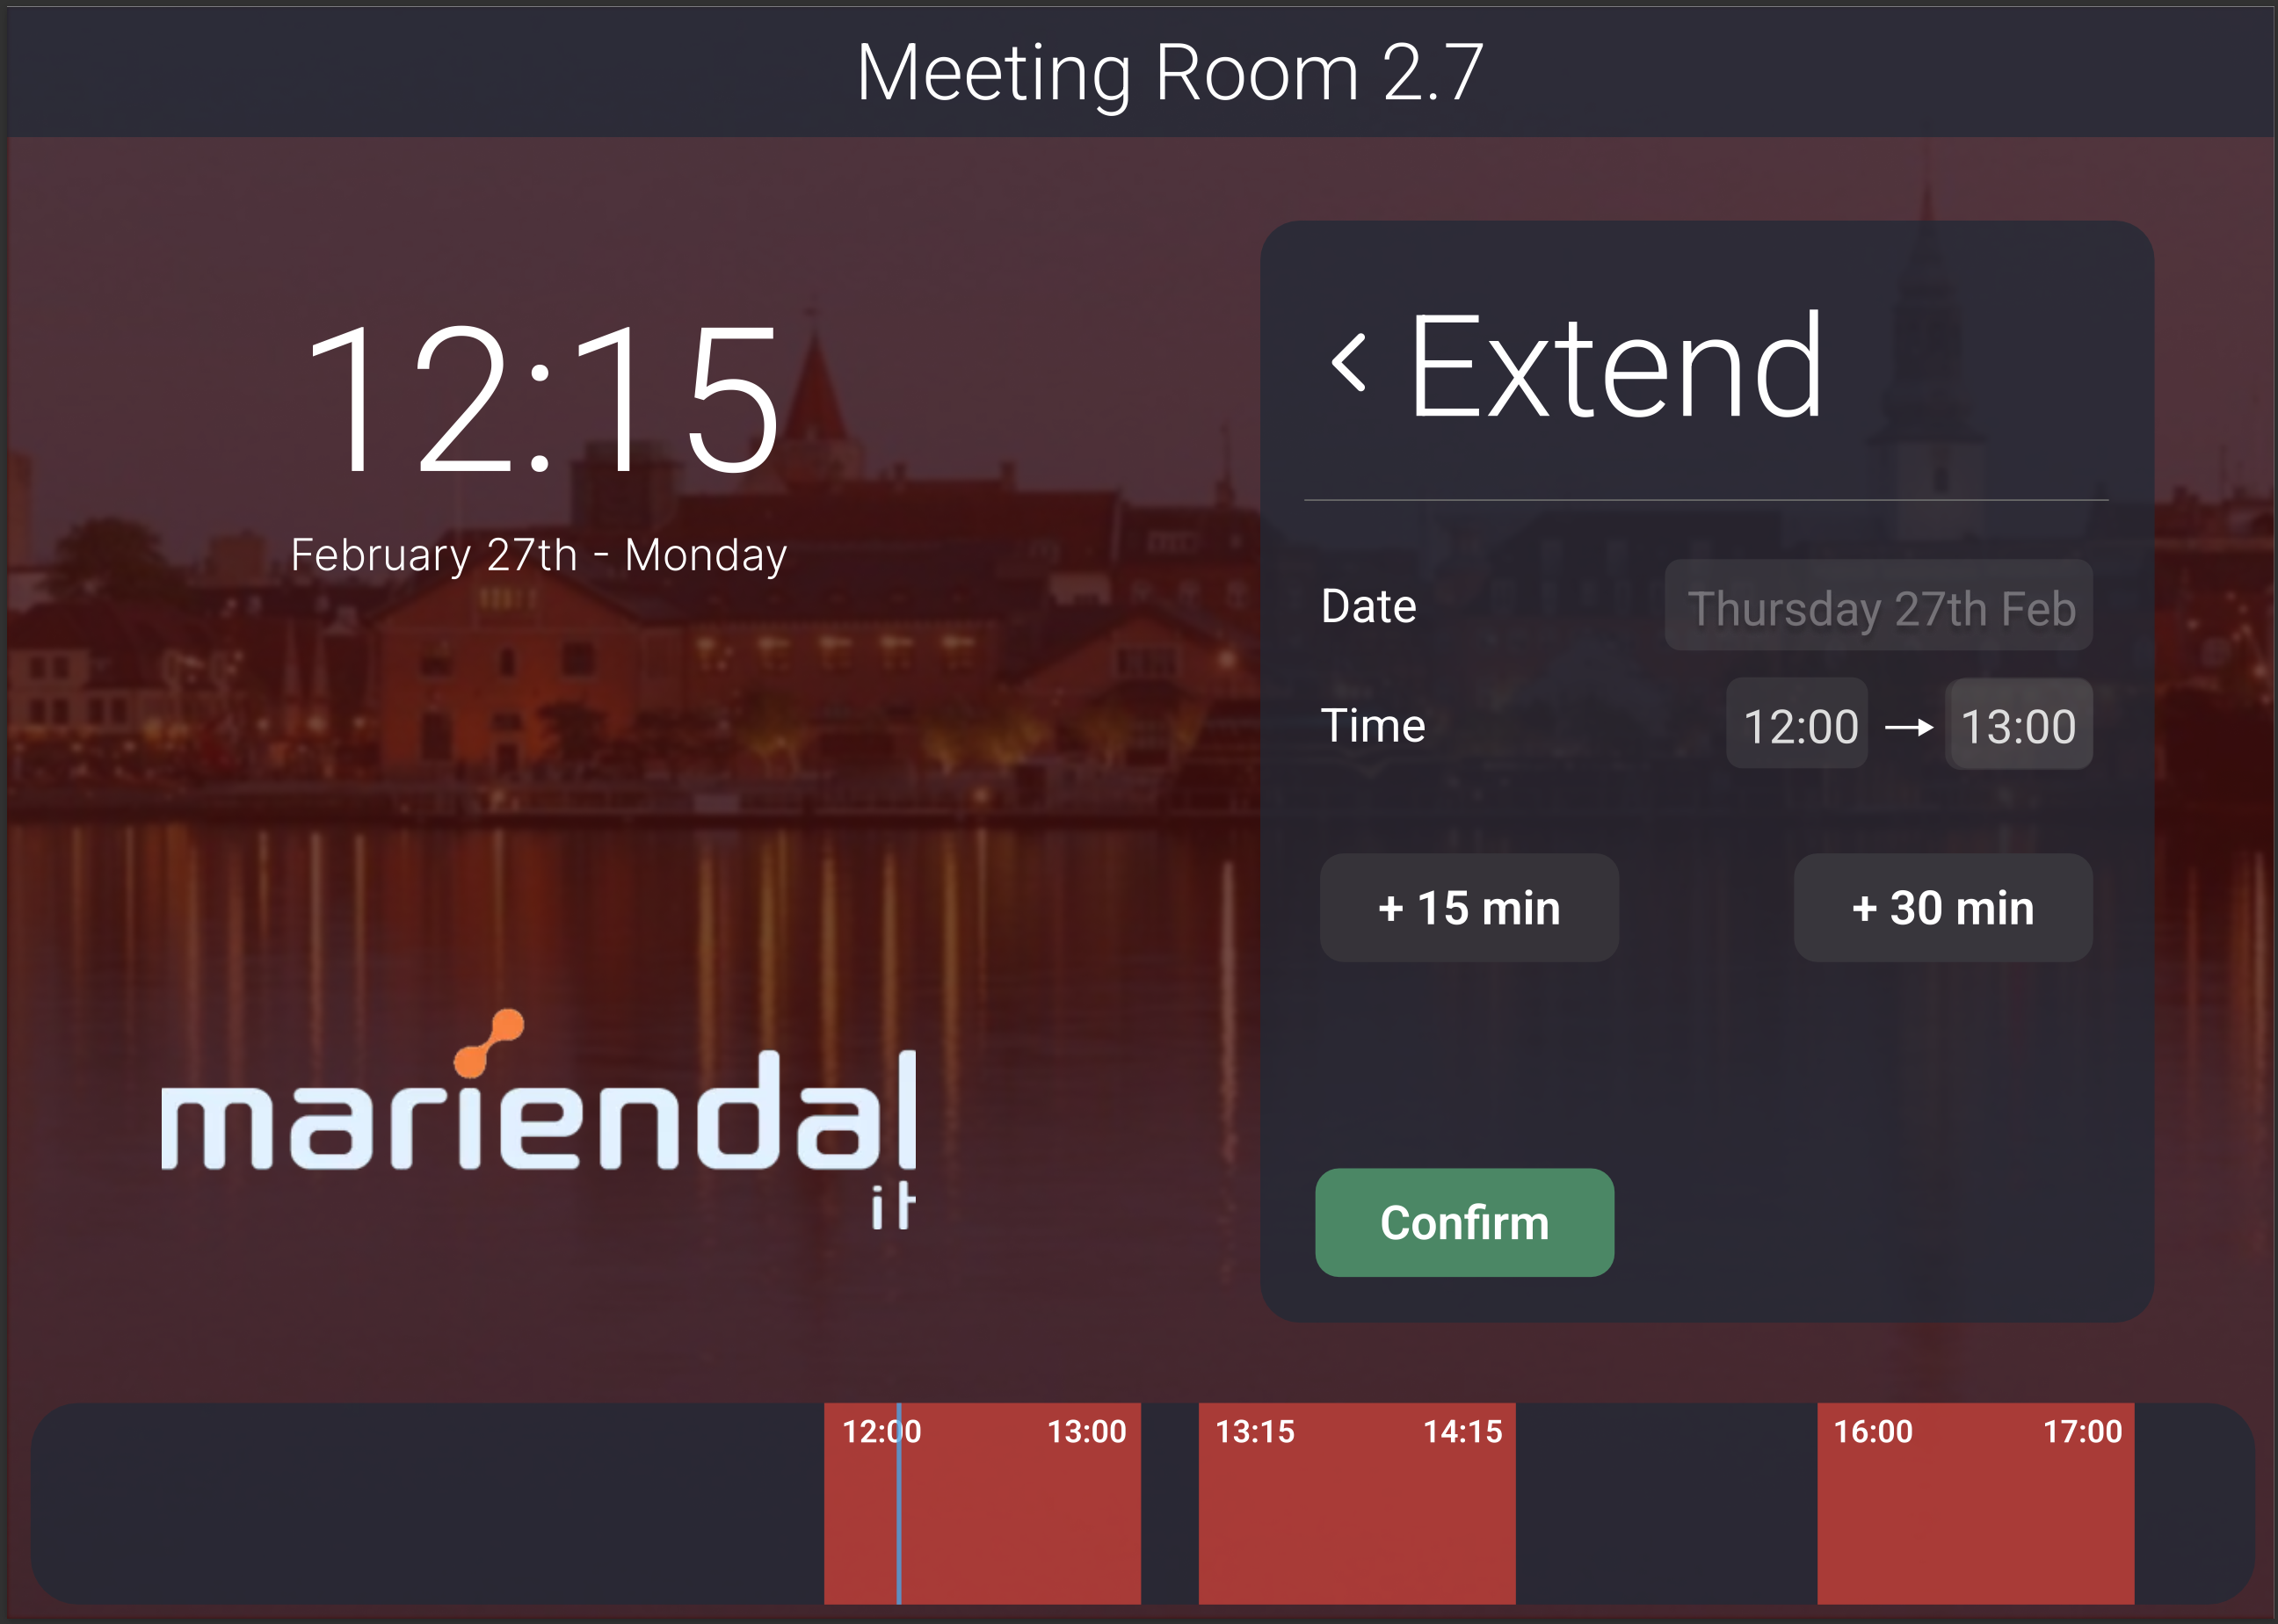
\includegraphics[width=1\textwidth]{images/occupied_extend_2.png}
    \caption{The occupied view with the extend action open on the right side.}
    \label{fig:occupied_extend2}
  \end{figure}

